下面进行指标的统计描述分析:主要是对上部分构造的球队数据进行统计描述。


%插入图片
\begin{enumerate}
	\item {\bfseries 球队胜率 球队胜率W/L\%}胜率的分布图如左图\ref{fig:2},可以看出胜率是近似的正态分布,轻微右偏,是轻尾的正态分布函数。根据右图\ref{fig:3}可知,在设定置信水平为95\%的情况下,正态分布和实际数据的点共同在蓝色置信带中,并且围绕在正态分布直线的两侧;
	\begin{figure}[h]
		
		\begin{subfigure}{0.5\textwidth}
			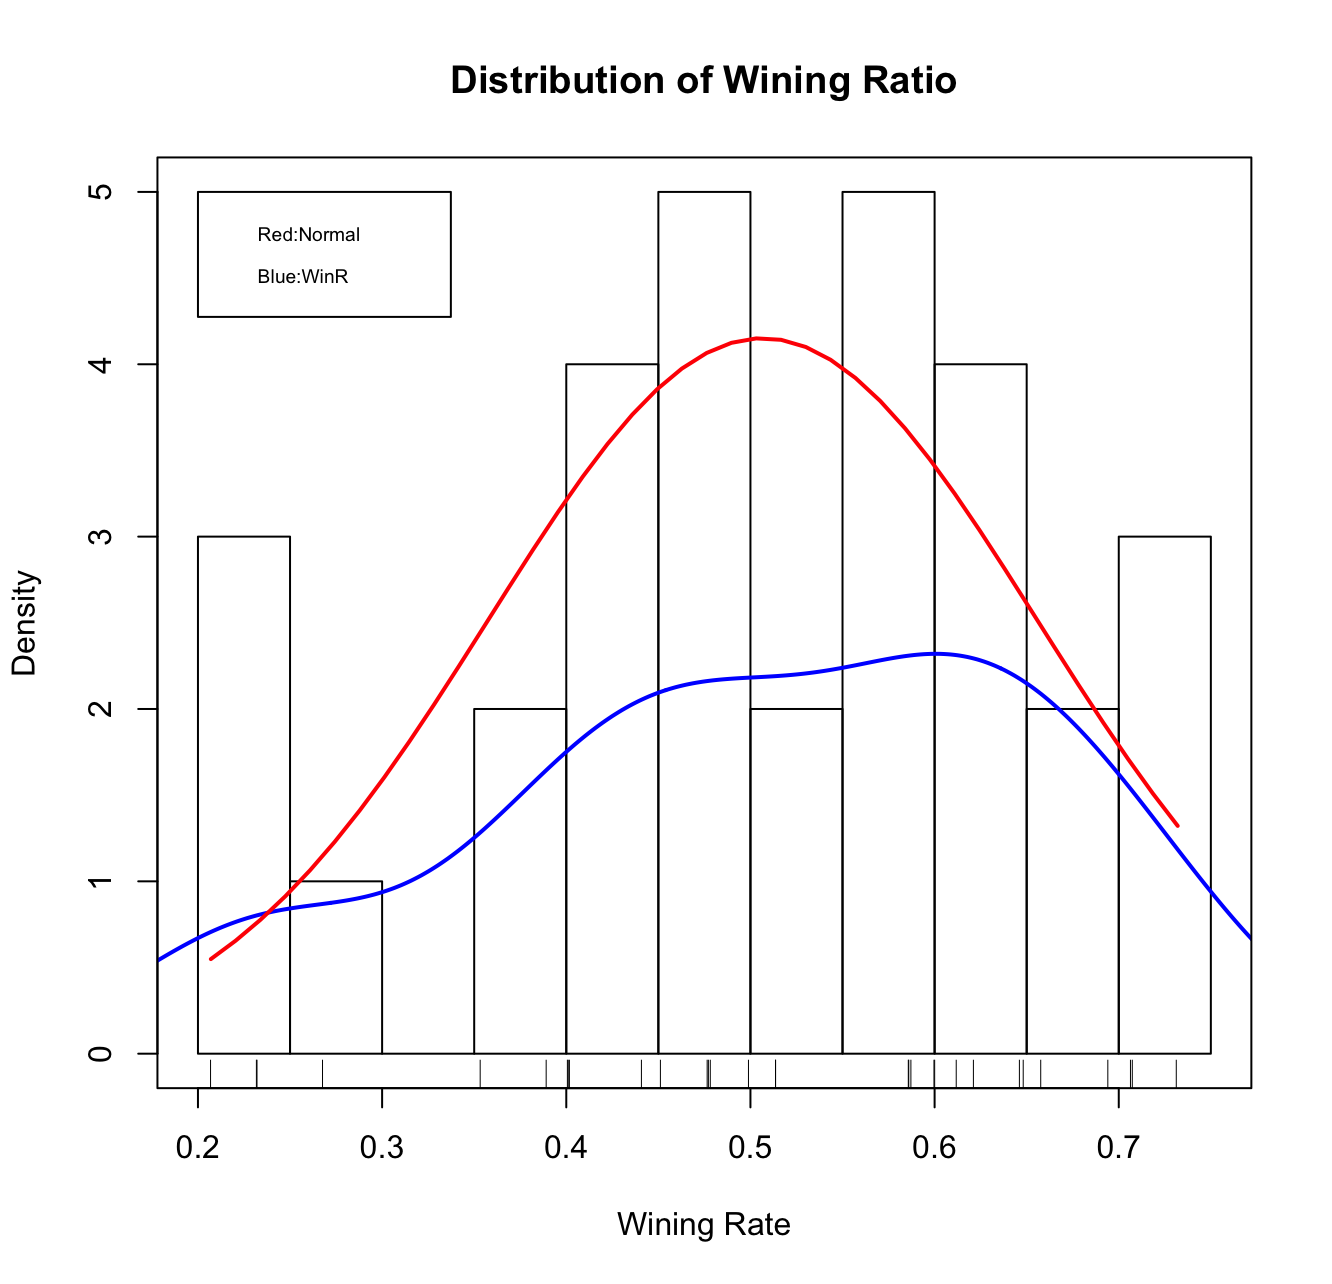
\includegraphics[width=0.9\linewidth, height=5cm]{distribution.png} 
			\caption{胜率分布图}
			\label{fig:2}
		\end{subfigure}
		\begin{subfigure}{0.5\textwidth}
			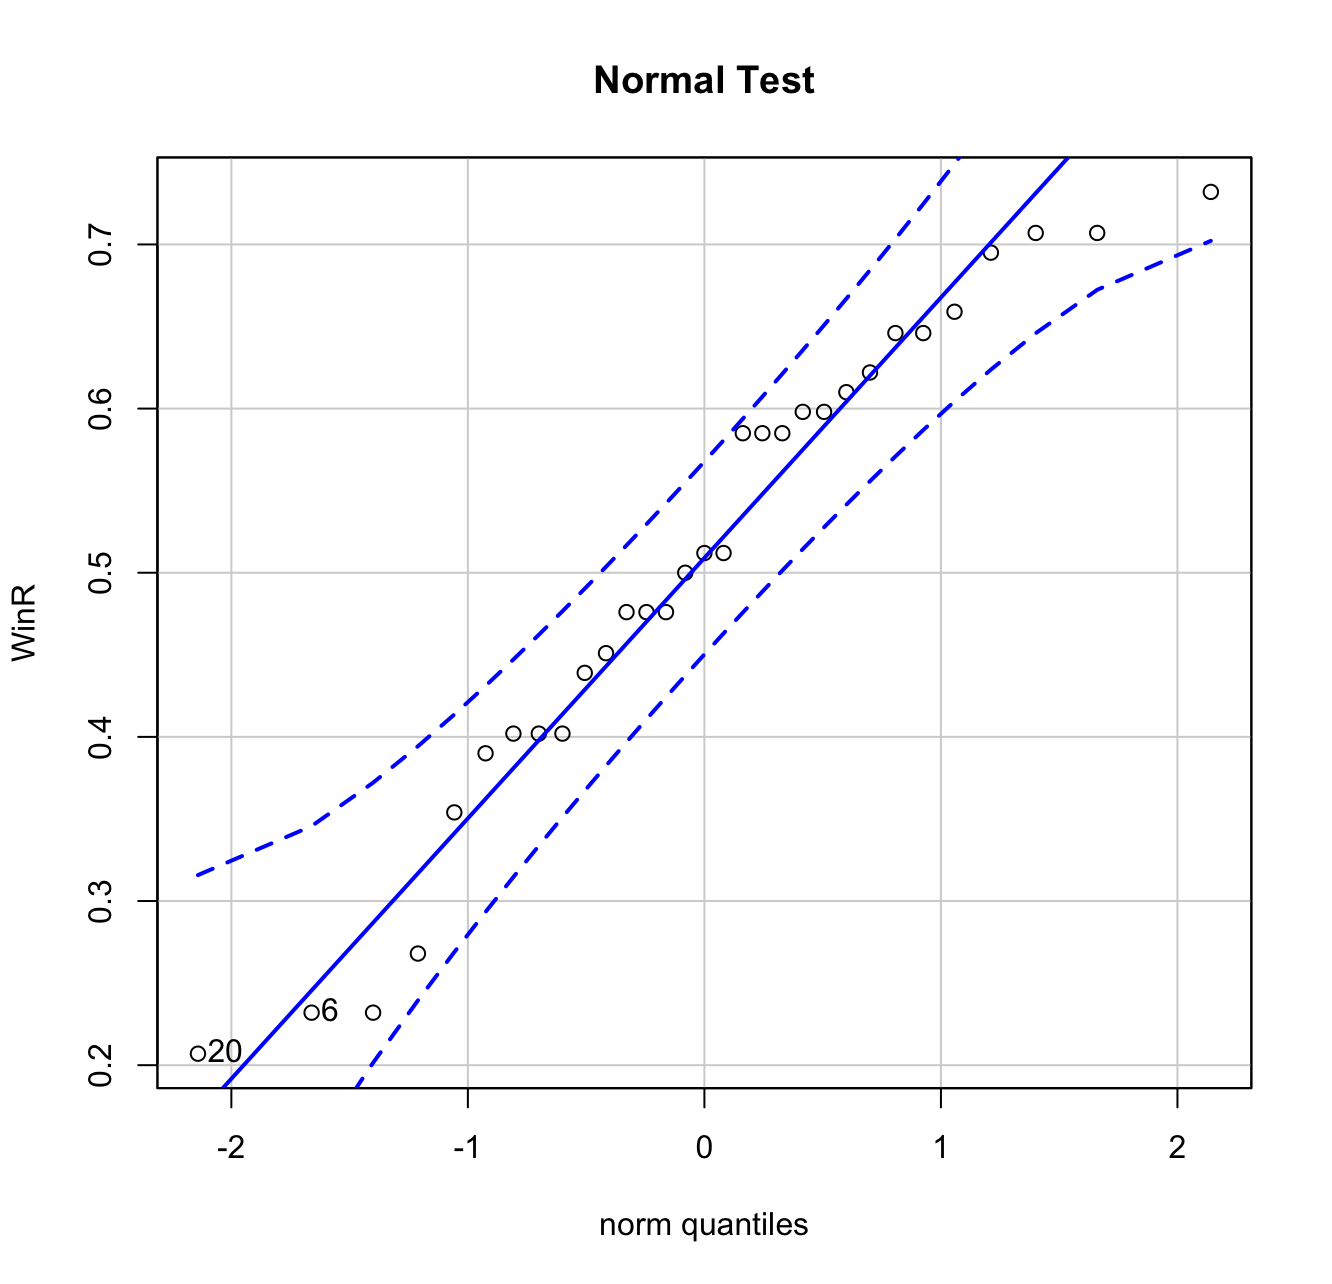
\includegraphics[width=0.9\linewidth, height=5cm]{NormTest}
			\caption{正态检验图}
			\label{fig:3}
		\end{subfigure}
	\caption{胜率统计描述图}
	\end{figure}
	在建模中希望数据服从近似正态分布,所以应对数据进行近一步正态性检验。
	利用Shapino-Wilks正态性检验,零假设为该样本符合正态分布,可看到如下表 $p=0.14>0.1$ ,可知在置信度为95\%水平下无法拒绝原假设,不能推翻样本的正太性假设。

	%正太性检验结果
	\begin{table}[h!]
			\begin{tabular}{|c|c|}
			\hline
			\multicolumn{2}{|c|}{Shapiro-Wilk normality test} \\
			\hline
			\multicolumn{2}{|c|}{ data:  data\$`W/L\%`} \\
			\hline
			W = 0.94857 &p-value = 0.1425\\
			\hline
		\end{tabular}
	\centering
	\label{4}
	\caption{正太性检验}
	\end{table}

%第二个变量	
	
\begin{figure}[h!]
	
	\begin{subfigure}{0.5\textwidth}
		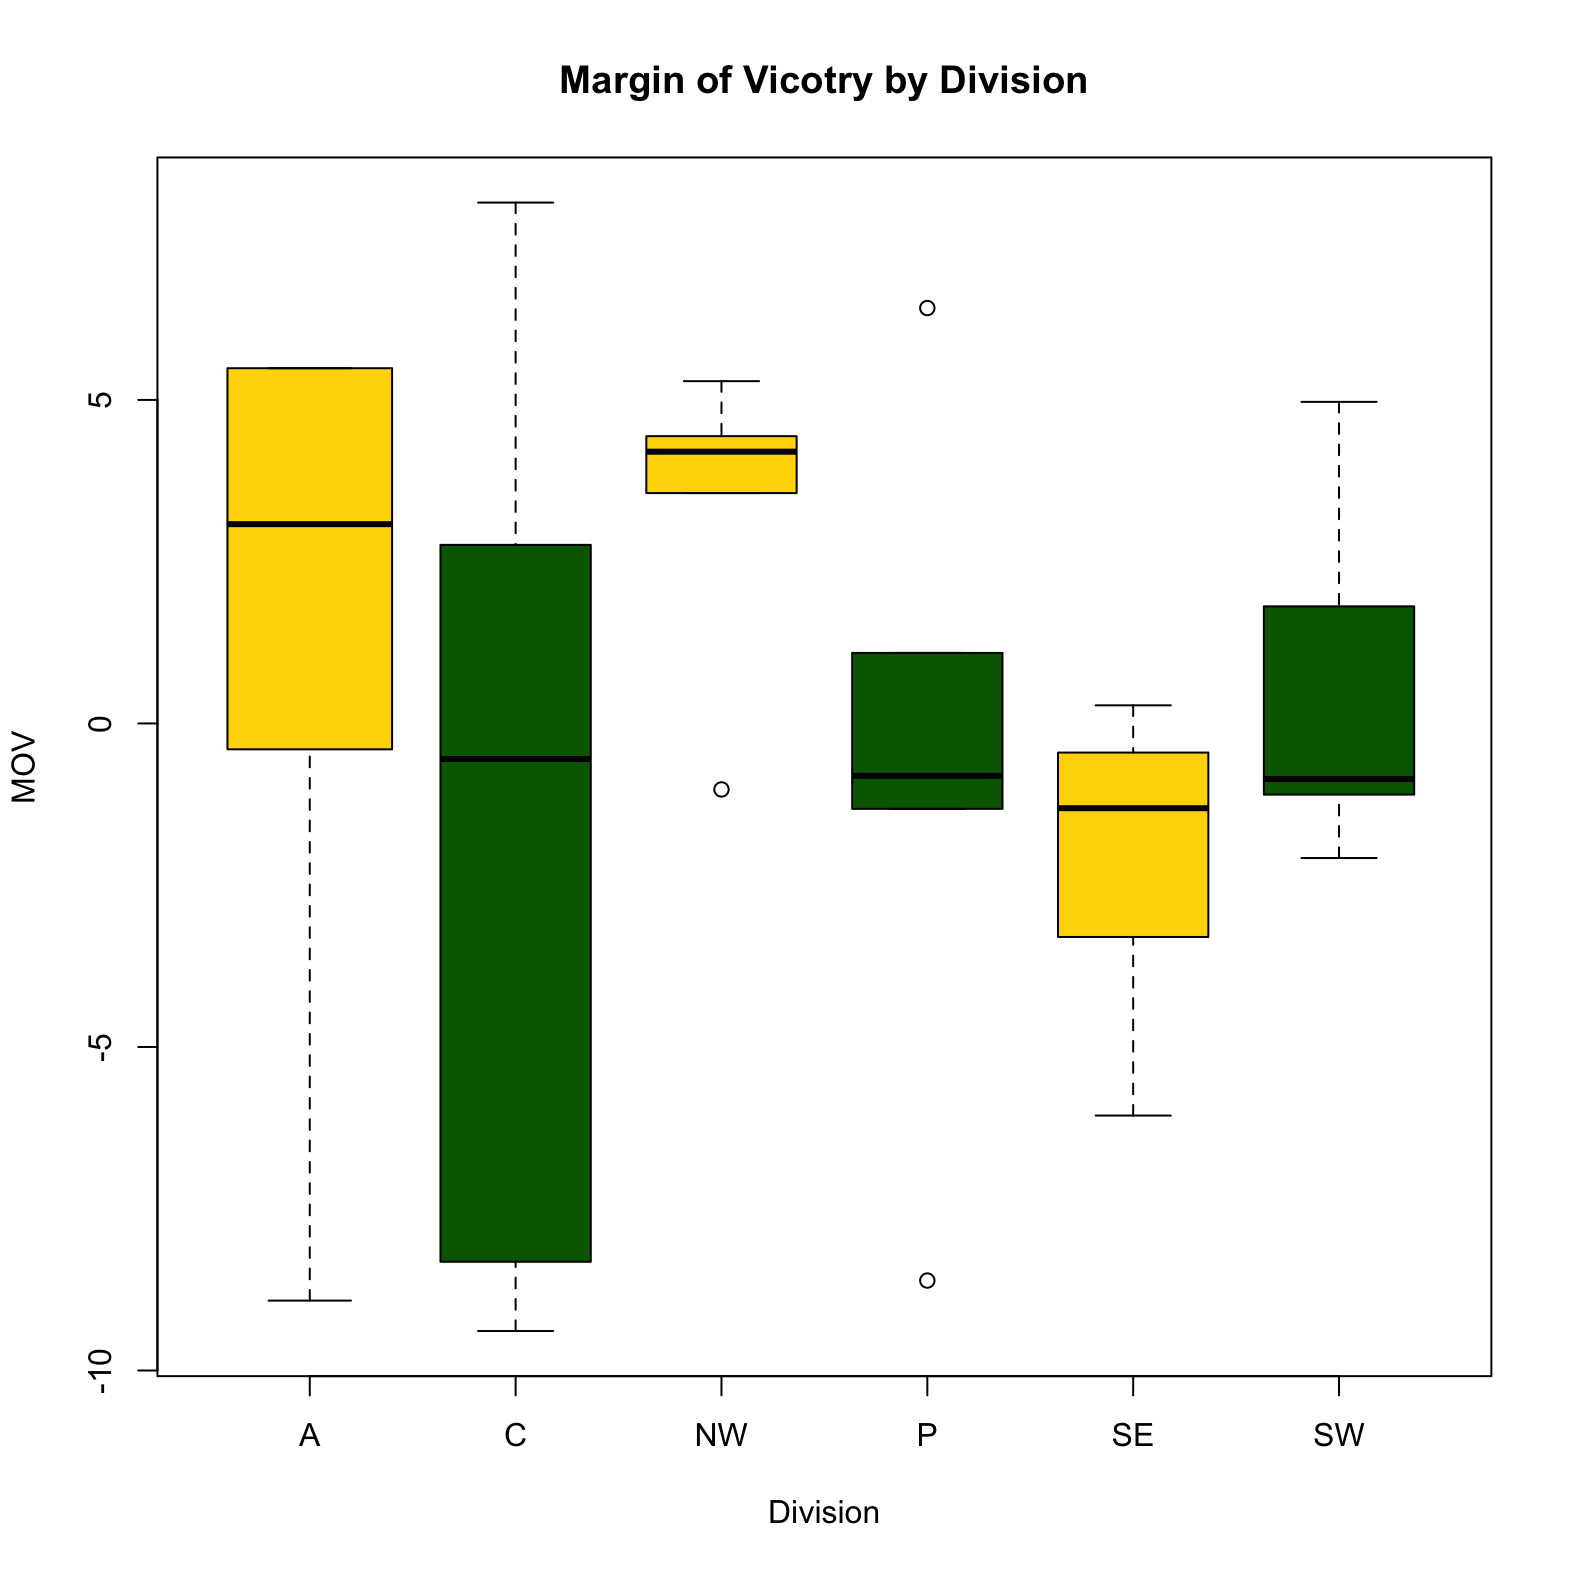
\includegraphics[width=0.9\linewidth, height=5cm]{MOVbp.png} 
		\caption{MOV的箱线图}
		\label{fig:4}
	\end{subfigure}
	\begin{subfigure}{0.5\textwidth}
		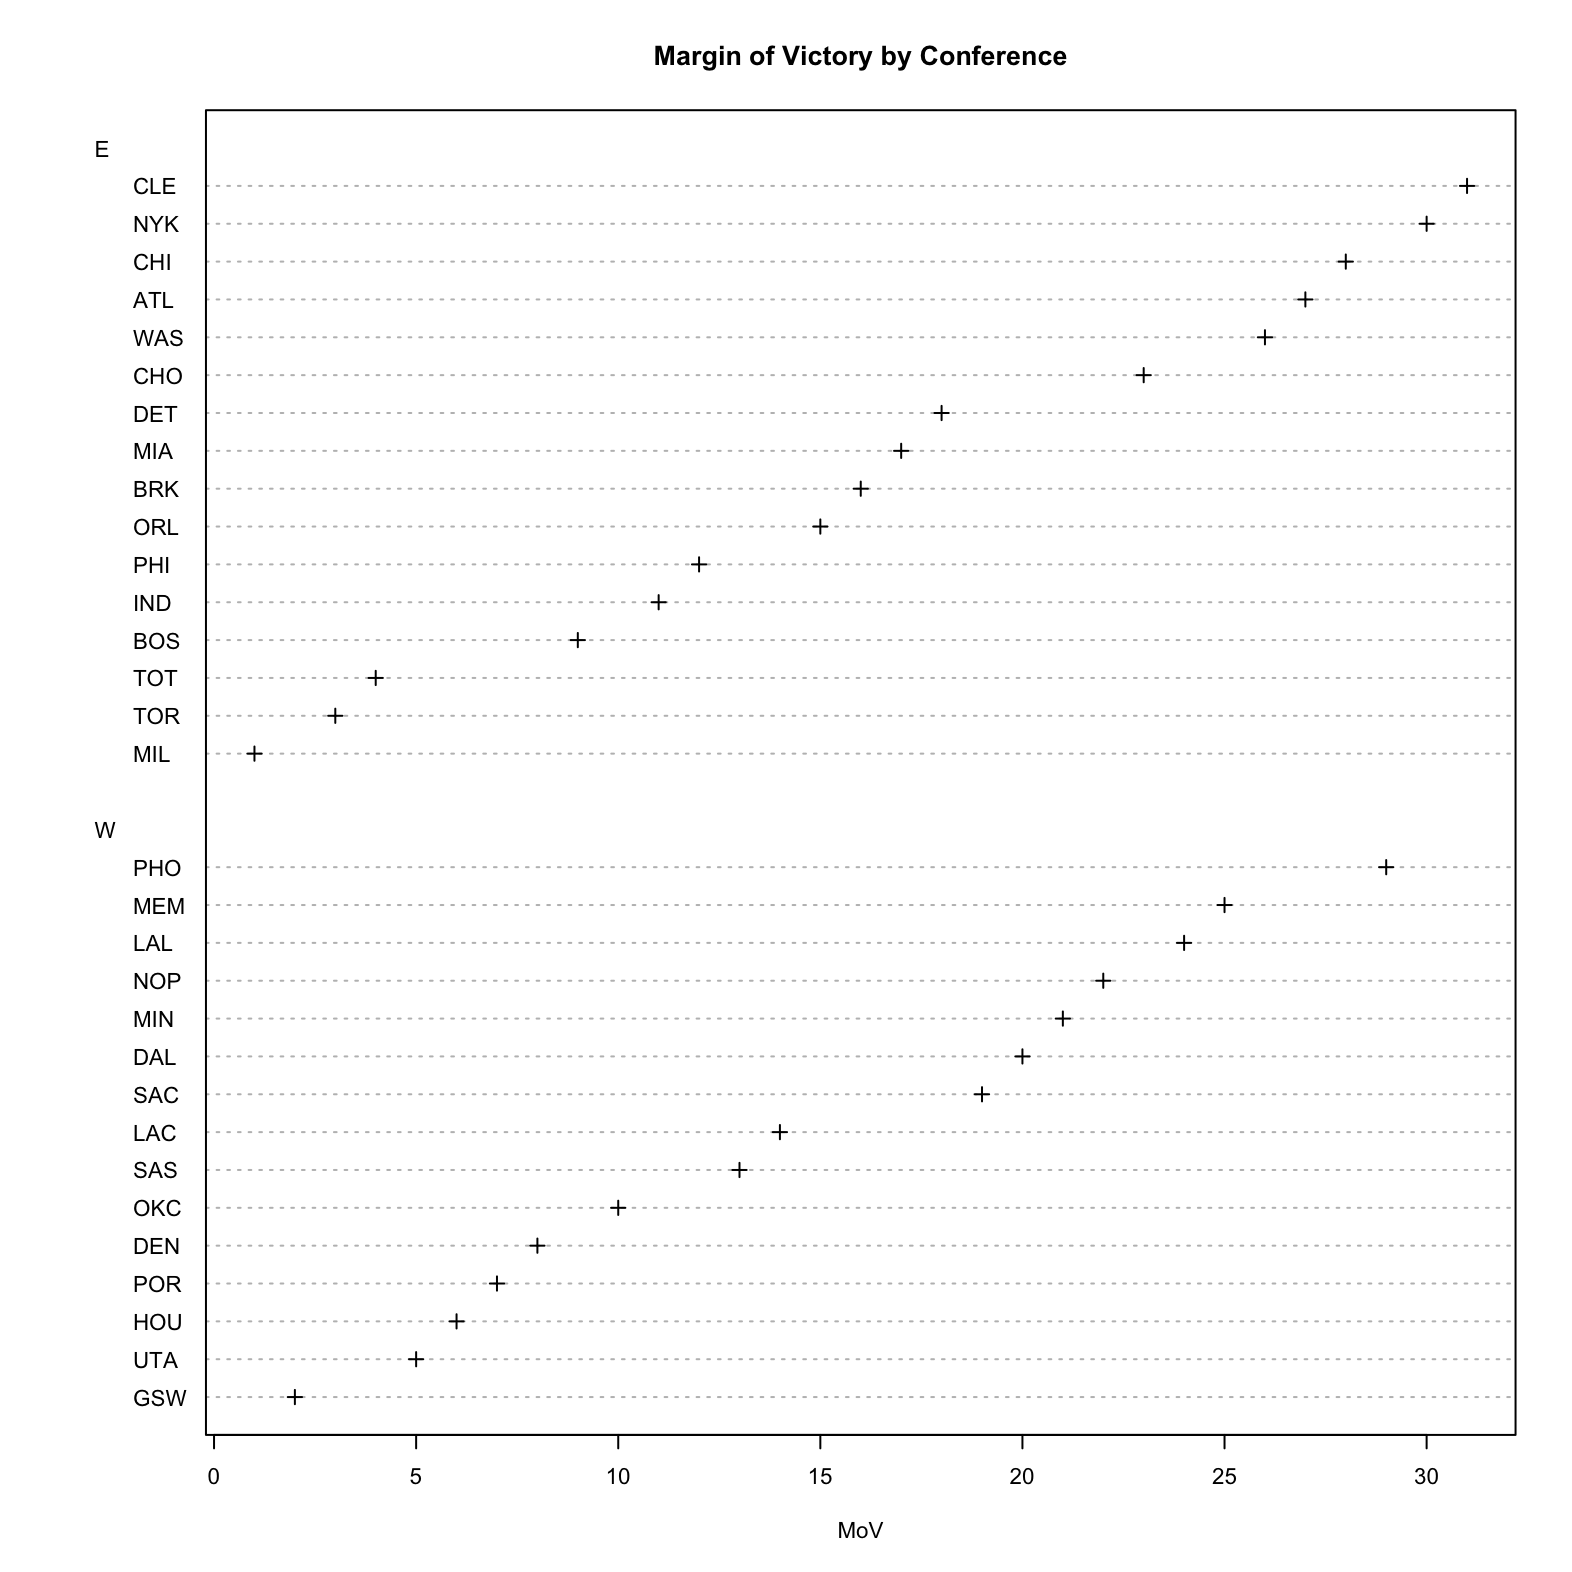
\includegraphics[width=0.9\linewidth, height=5cm]{Movdotp.png}
		\caption{MOV的散点图}
		\label{fig:5}
	\end{subfigure}
\caption{比分差距统计描述}
\end{figure}
	\item  {\bfseries 比分差距MOV/A的描述性分析:}左图\ref{fig:4}详细描绘了每个地区的比分差距变量的分布情况,其中比分差距变量分布最离散的是中部地区,涵盖了比分差距变量的最大值和最小值,西北地区的比分差距变量离散程度最小,数据最集中。亚特兰大地区和西北地区的球队比分差距变量基本位正,说明这些地区的球队实力很强;右图\ref{fig:5}详细列出了东部地区和西部地区所有队伍的比分差距的排名情况,其中比分差距最高的球队是东部地区的克利夫兰骑士队,比分差距最低的队伍是东部地区的密尔沃基雄鹿队。
%第三个变量

\item {\bfseries 进攻效率ORtg/A的描述性分析:  }左图\ref{fig:6} 详细描绘了每个地区的进攻效率变量的分布情况,右图\ref{fig:7} 详细列出了东部地区和西部地区所有队伍的比分差距的排名情况,中部地区和东南部地区的球队进攻效率相对较低,其中太平洋地区的进攻效率较为离散,根据进攻效率可以看出球队的风格差异;右图详细列出了东部地区和西部地区所有队伍的进攻效率的排名情况,其中东部地区进攻效率相较西部地区更为优秀一些,东部地区进攻效率最高的球队是纽约尼克斯,这说明该球队的风格更偏向进攻。
\begin{figure}[h!]
	
	\begin{subfigure}{0.5\textwidth}
		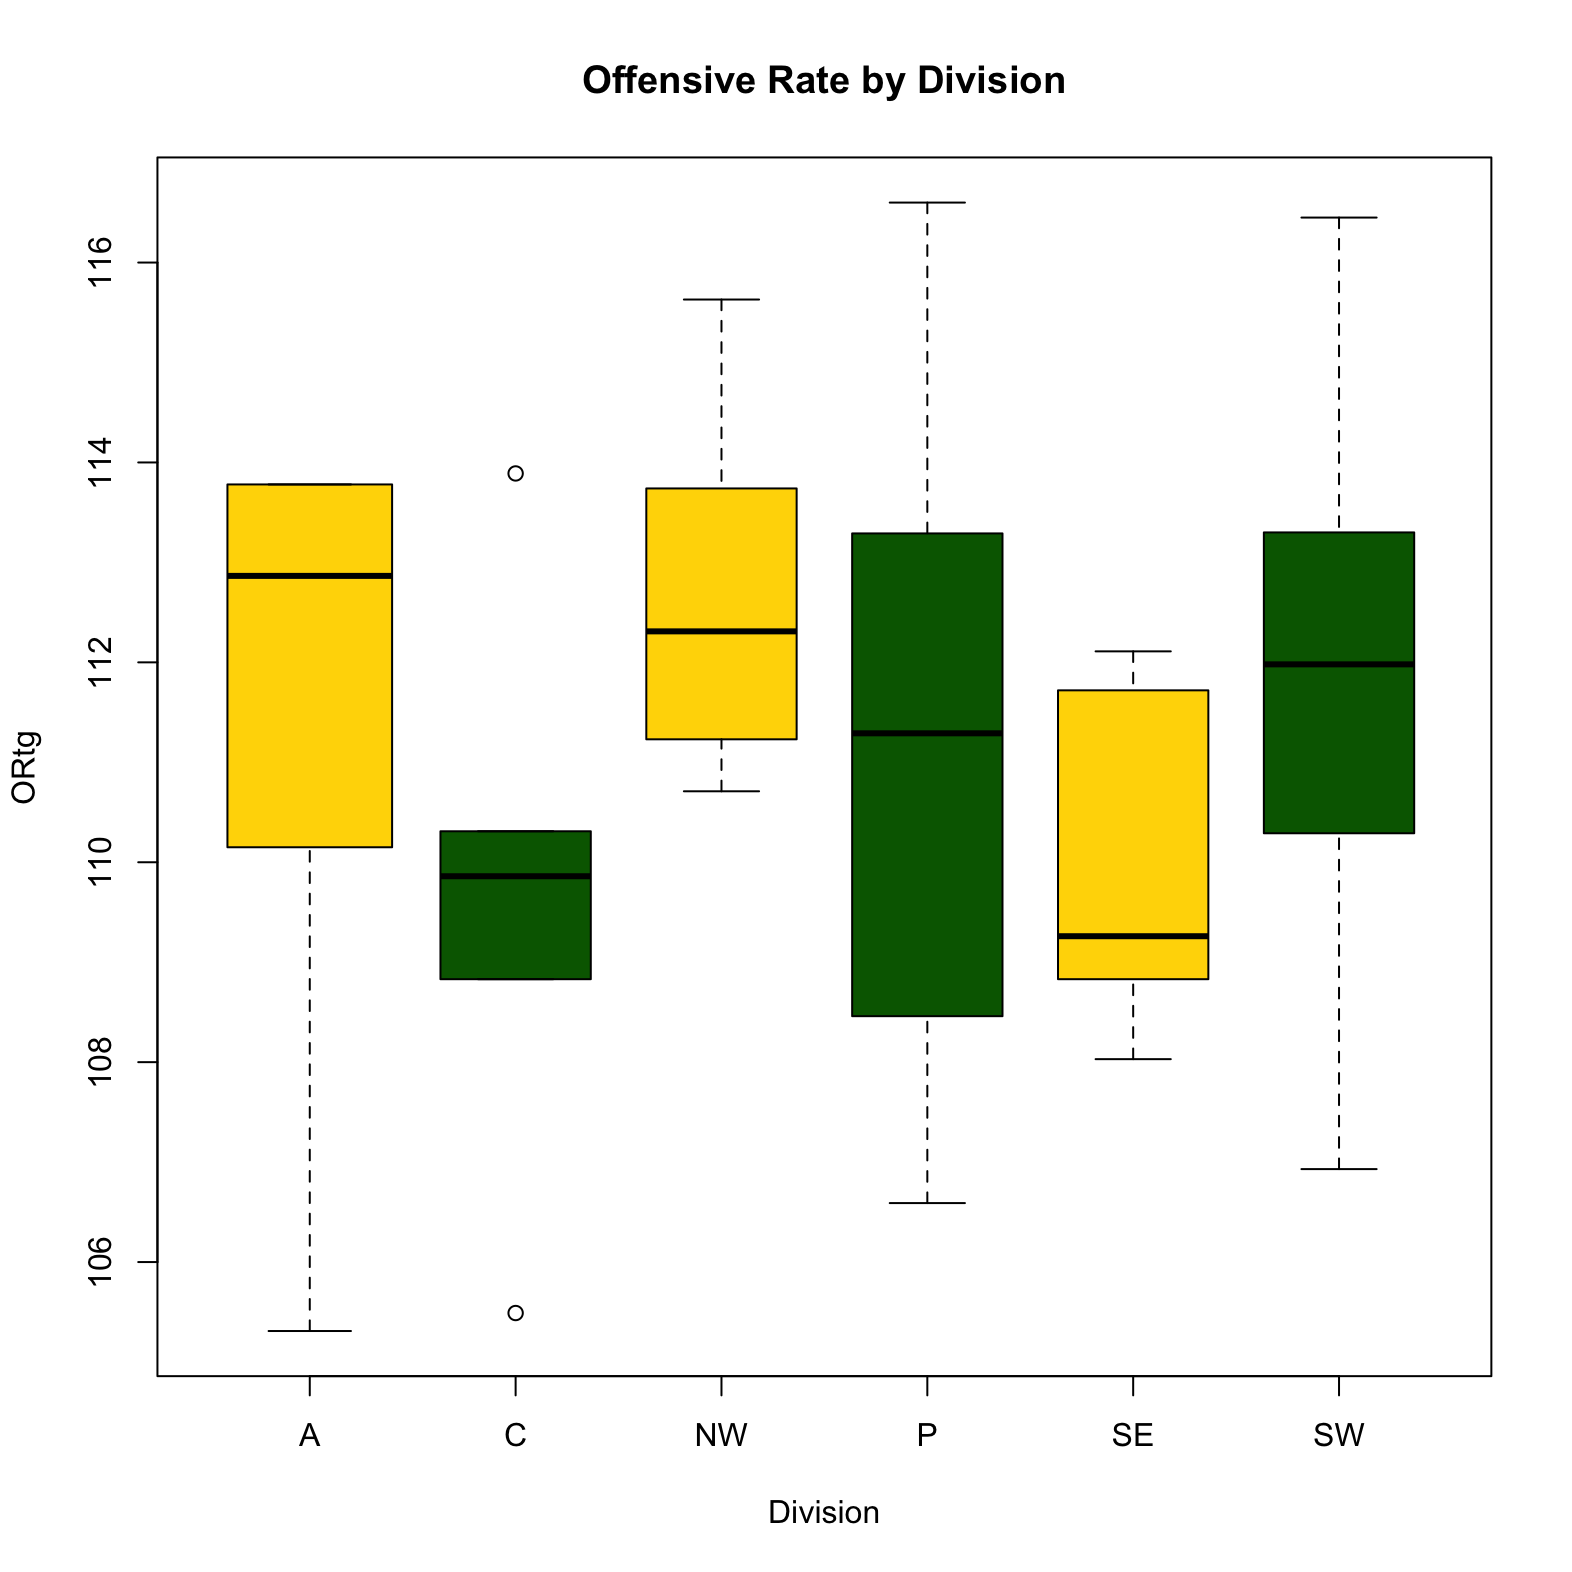
\includegraphics[width=0.9\linewidth, height=5cm]{ORgbp.png} 
		\caption{进攻效率箱线图}
		\label{fig:6}
	\end{subfigure}
	\begin{subfigure}{0.5\textwidth}
		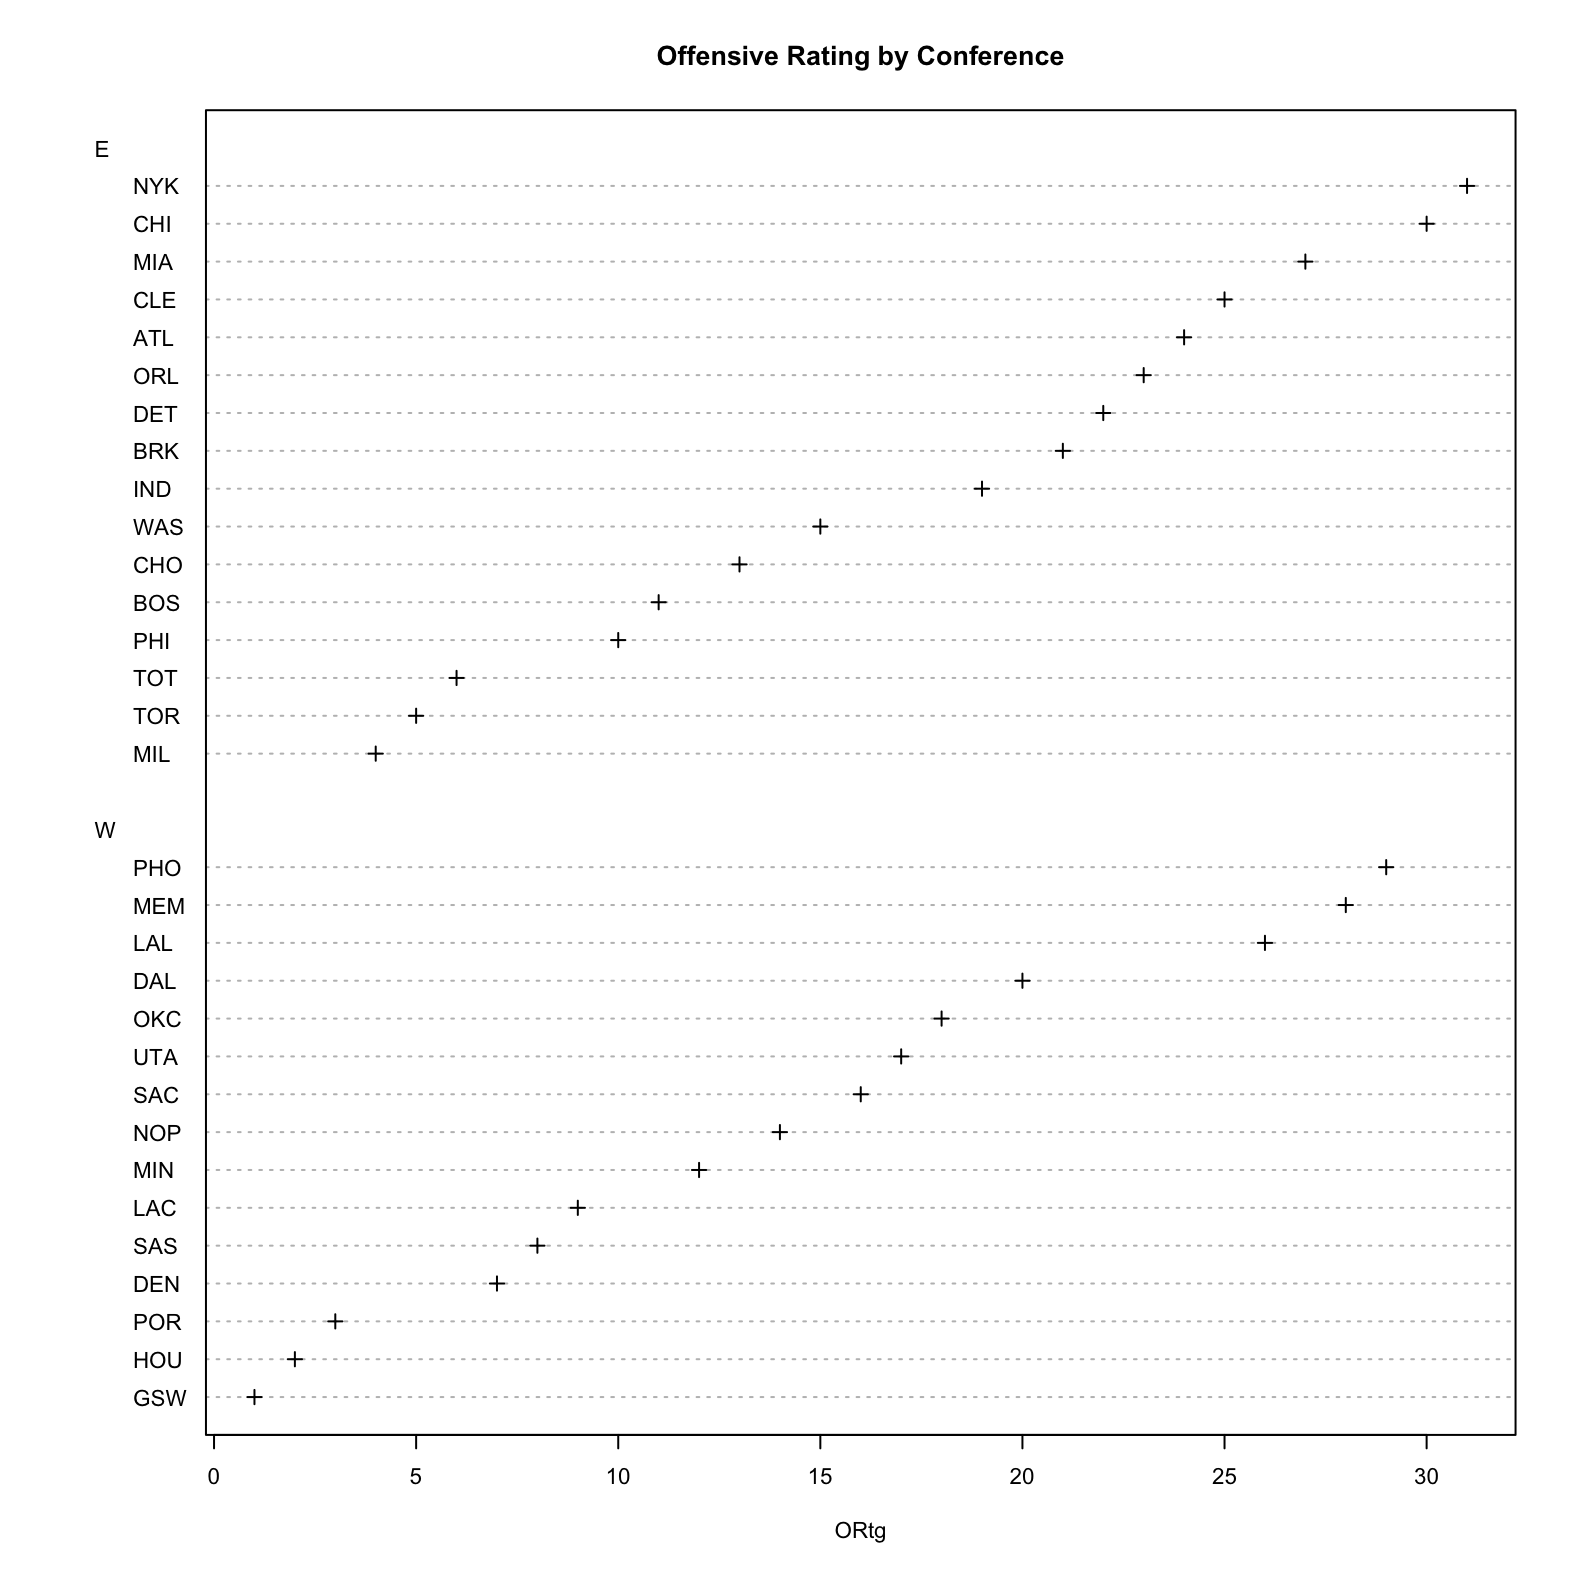
\includegraphics[width=0.9\linewidth, height=5cm]{ORtgdotp.png}
		\caption{进攻效率散点图}
		\label{fig:7}
	\end{subfigure}
	\caption{进攻效率统计描述}
\end{figure}


%第四个变量
\item {\bfseries 球员效率Team\_PER的描述统计}左图\ref{fig:8} 详细描绘了每个地区的球队的球员效率率变量的分布情况,西北部地区和西南部地区的球队的球员效率率指标分布较为集中,且这些地区的球员效率很高,即中位数是所有地区中最高的,上四分位数和下四分位数也是最高的,亚特兰大地区和东南部地区的球队球员效率变量分布较为离散;右图\ref{fig:9} 详细列出了东部地区和西部地区所有队伍球员效率变量的排名情况,东部地区的亚特兰大老鹰队球员效率最高,东部地区的费城76人队的球员效率最低。
\begin{figure}[h!]
	
	\begin{subfigure}{0.5\textwidth}
		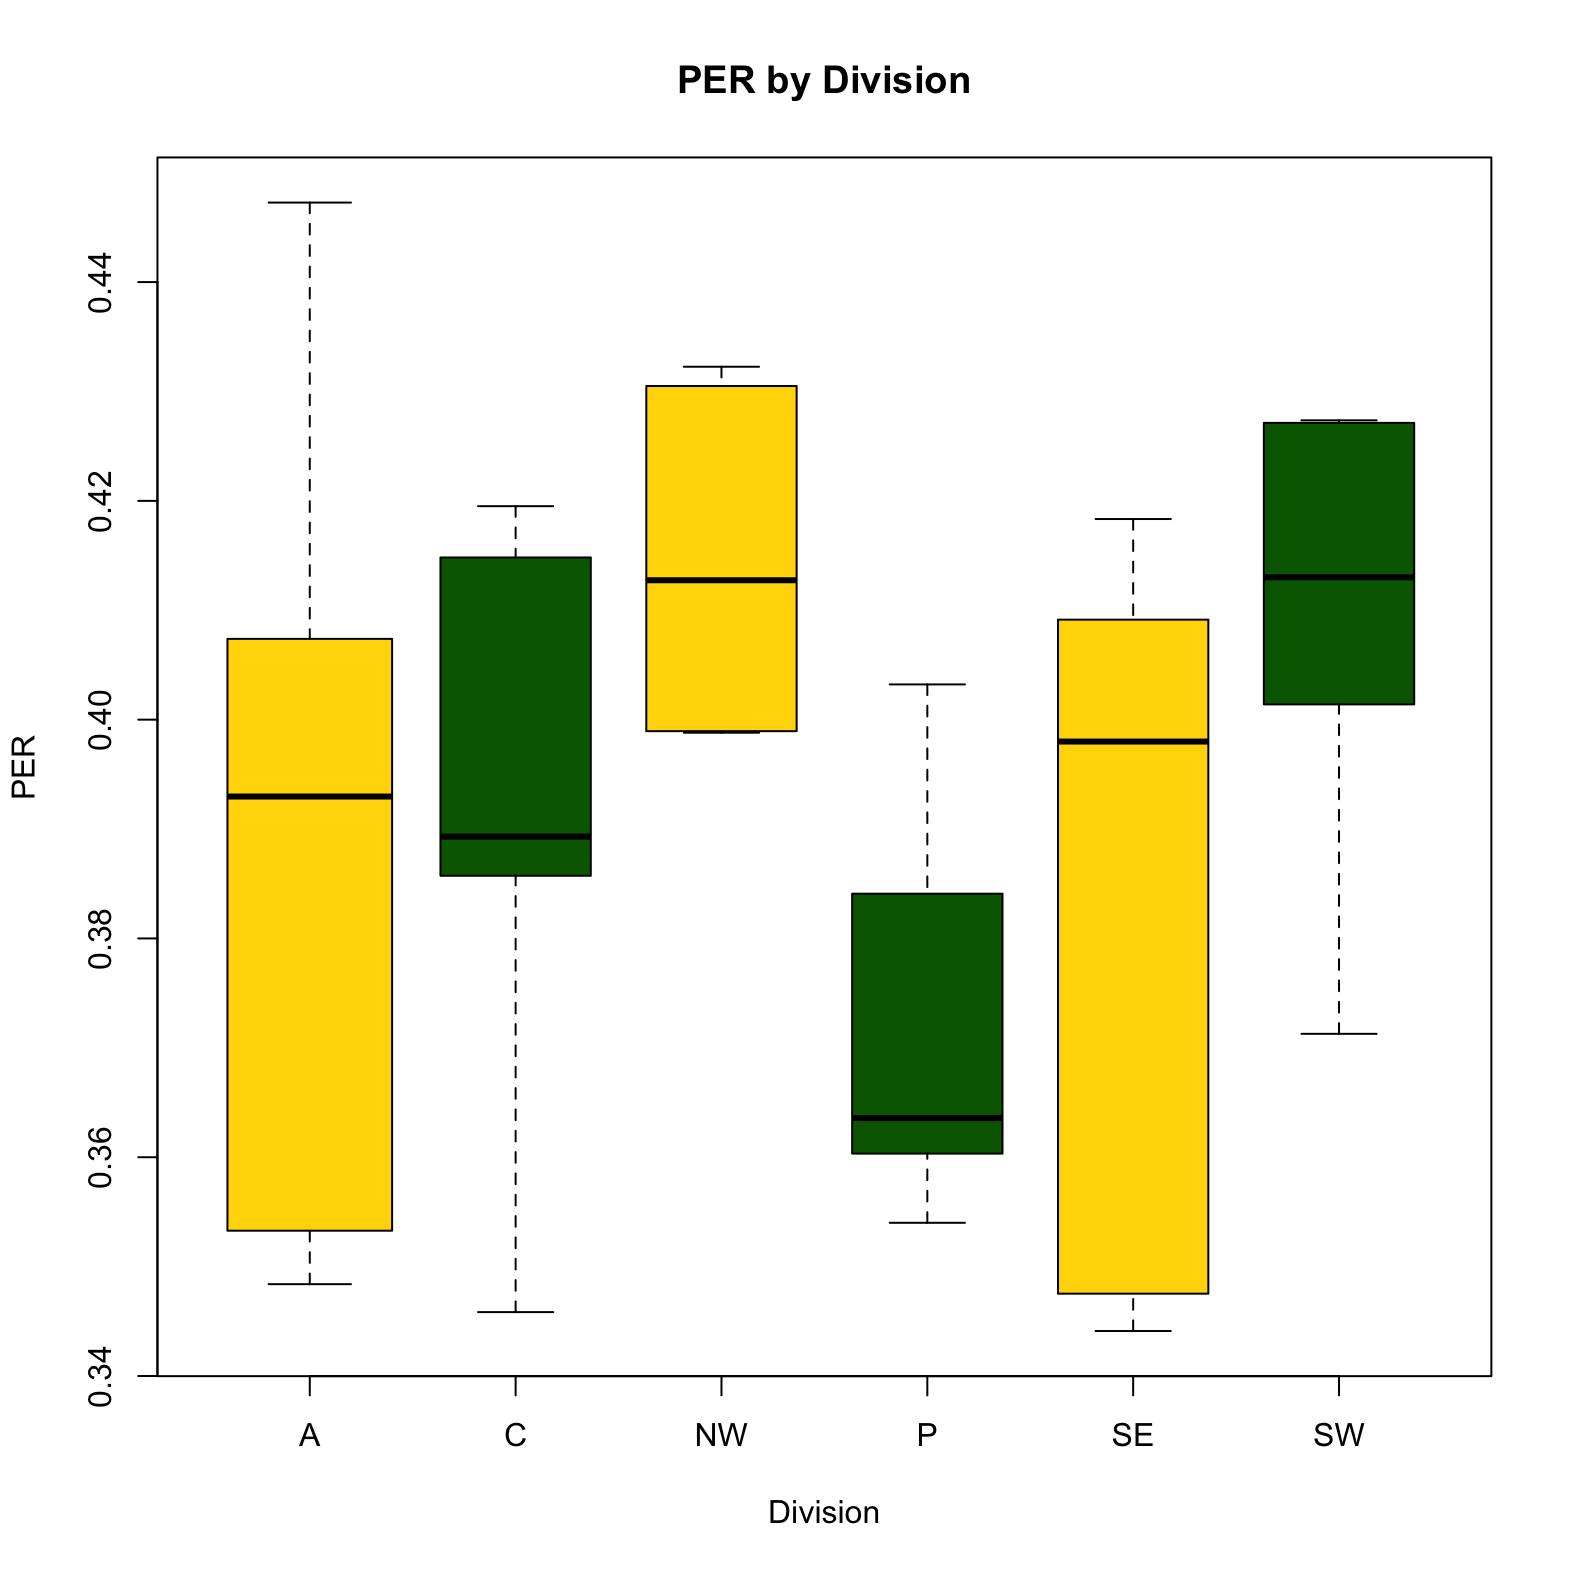
\includegraphics[width=0.9\linewidth, height=5cm]{PERbp.png} 
		\caption{球员效率箱线图}
		\label{fig:8}
	\end{subfigure}
	\begin{subfigure}{0.5\textwidth}
		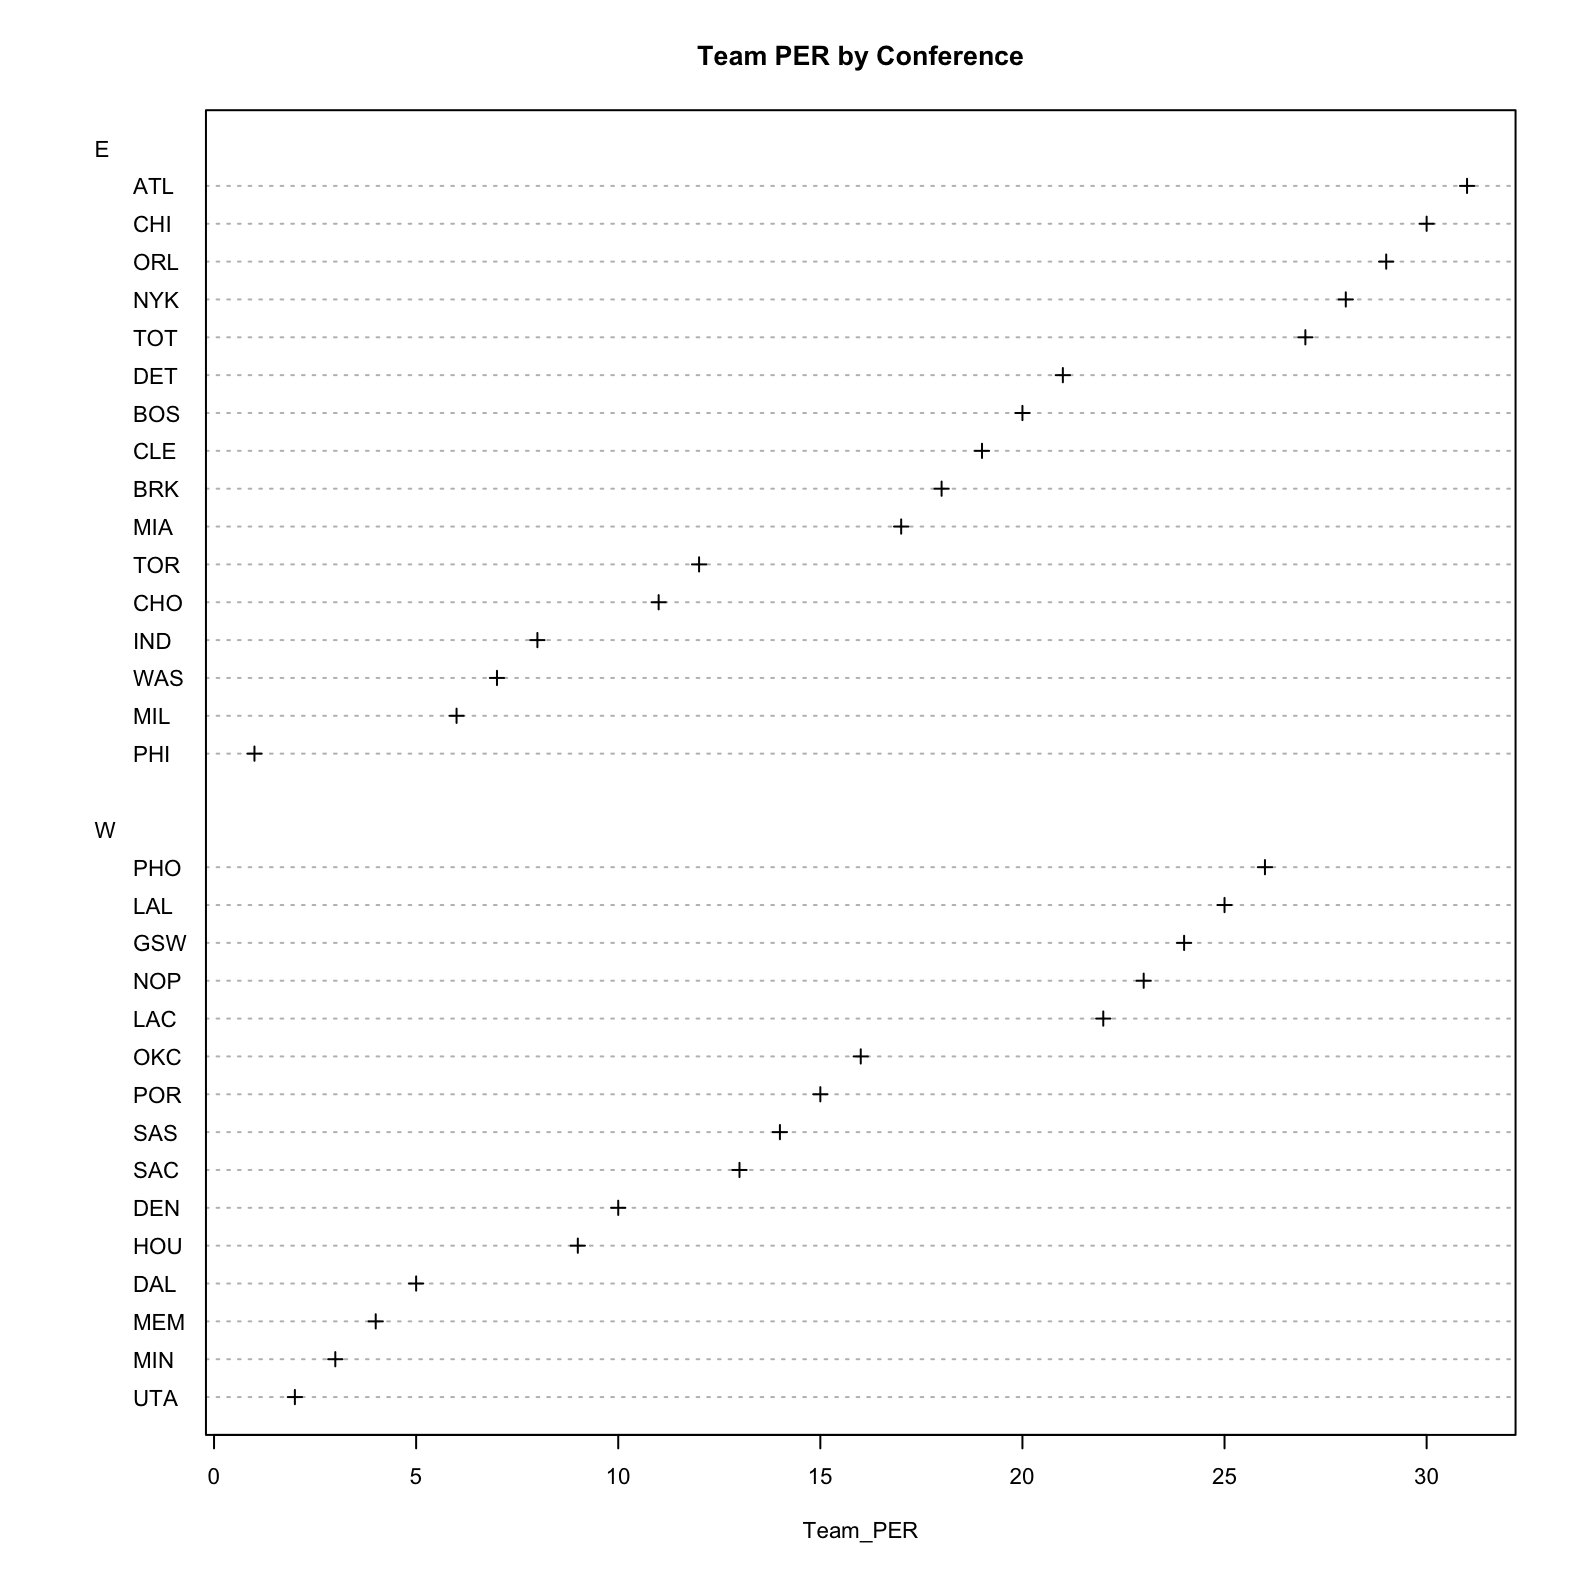
\includegraphics[width=0.9\linewidth, height=5cm]{PERdotp.png}
		\caption{球员效率散点图}
		\label{fig:9}
	\end{subfigure}
	\caption{球员效率统计描述}
\end{figure}

%第五个变量
\newpage
\item {\bfseries 球员有效得分率 Team\_eFGP的统计描述}左图\ref{fig:10}详细描绘了每个地区的球队的球员有效得分率的分布情况,可以看出各个地区球队球员有效得分率的中间水平都在0.4附近,其中太平洋地区的球队球员的有效得分率中位数最低,西南地区球队的球员有效得分率分布最离散;右图\ref{fig:11}详细列出了东部地区和西部地区所有队伍球员效率变量的排名情况,东部地区的球员有效得分率最高的球队是CHI,NYK,TOT,芝加哥公牛,多伦多猛龙队,纽约尼克斯队。东部球队的球员有效得分率相对西部球队较高。

\begin{figure}[h!]
	
	\begin{subfigure}{0.5\textwidth}
		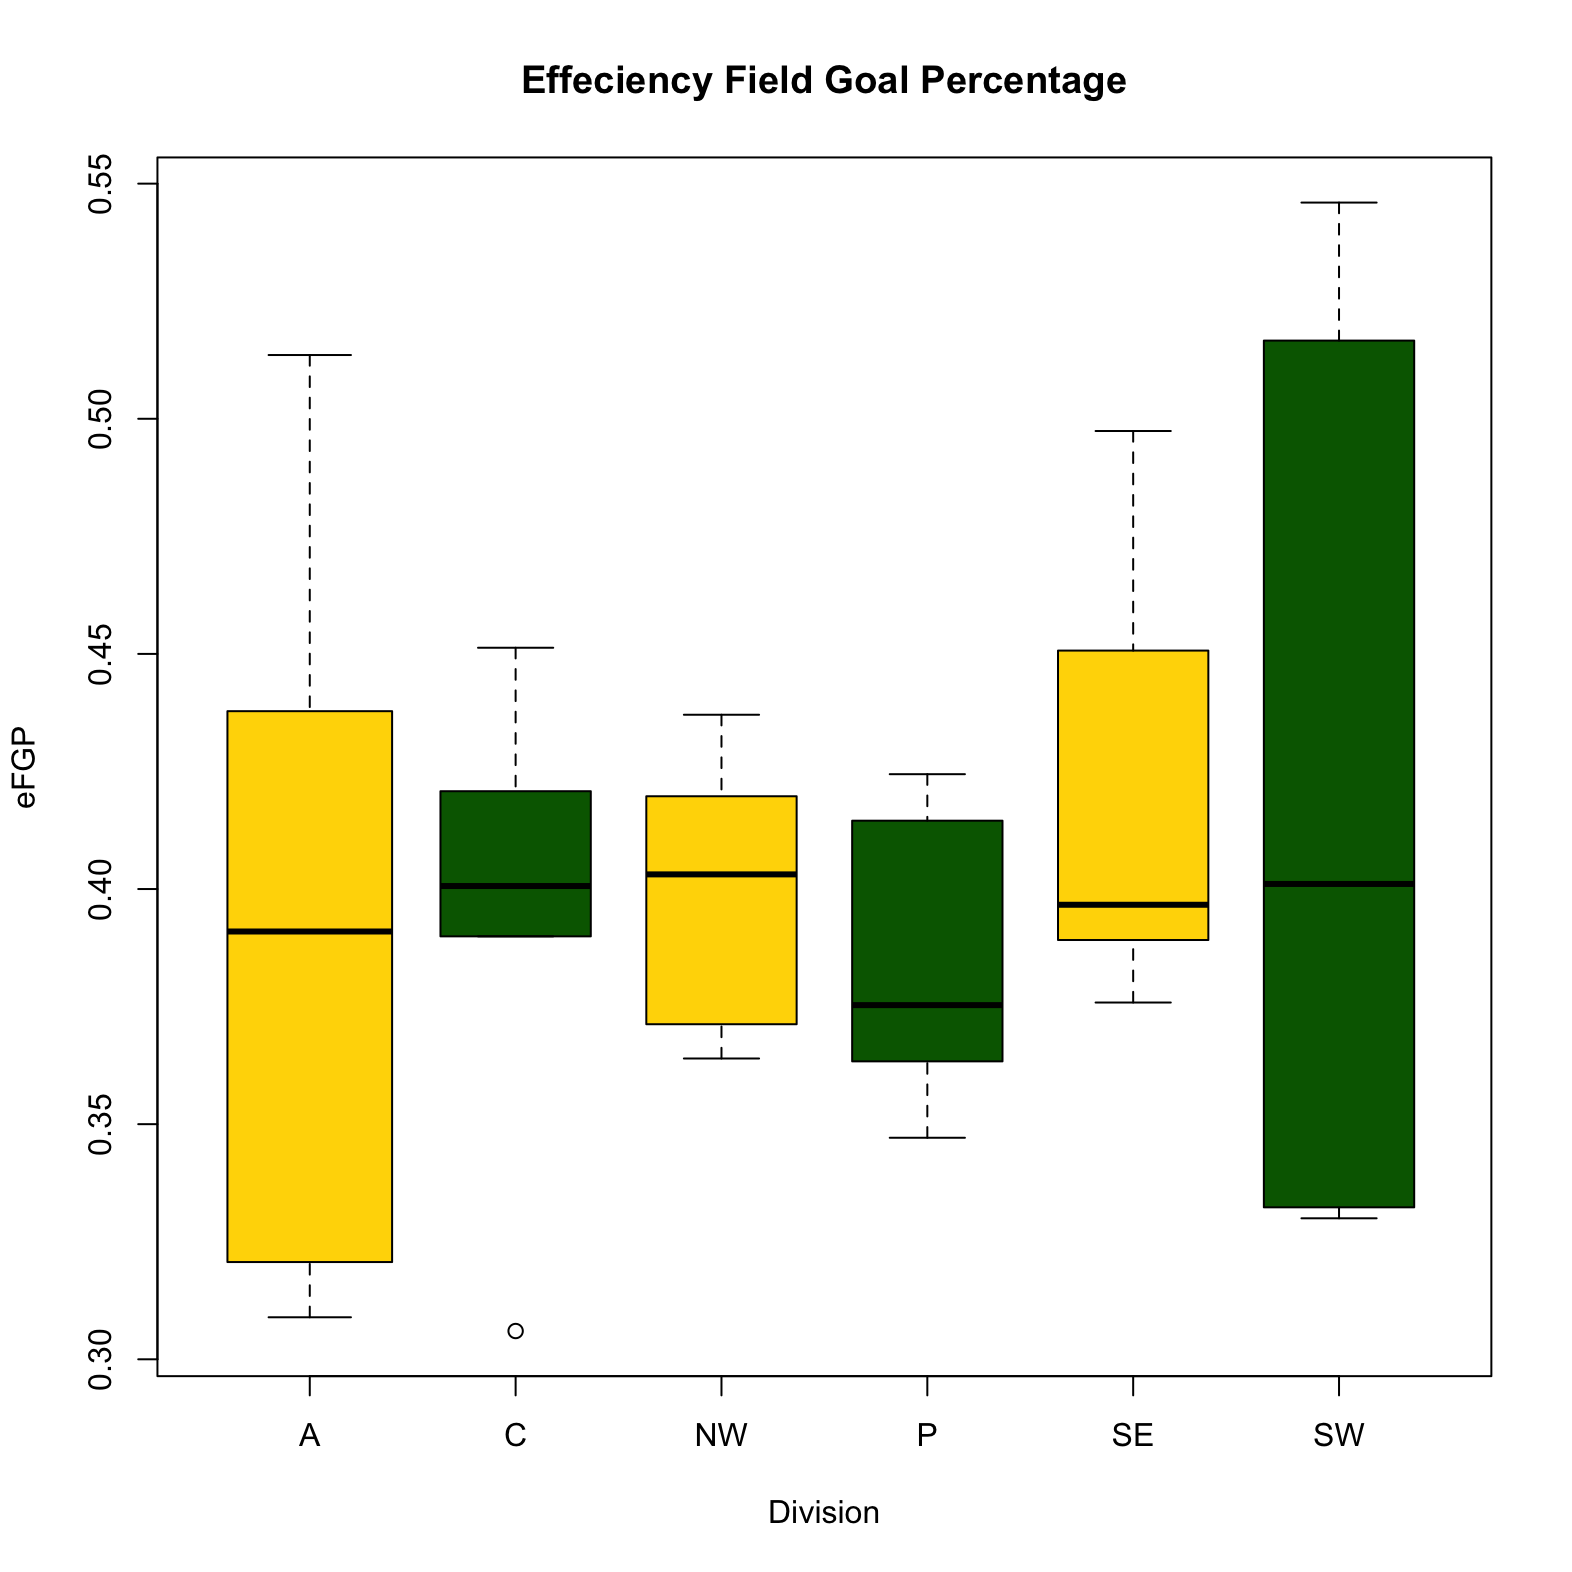
\includegraphics[width=0.9\linewidth, height=5cm]{eFGP.png} 
		\caption{有效得分率箱线图}
		\label{fig:10}
	\end{subfigure}
	\begin{subfigure}{0.5\textwidth}
		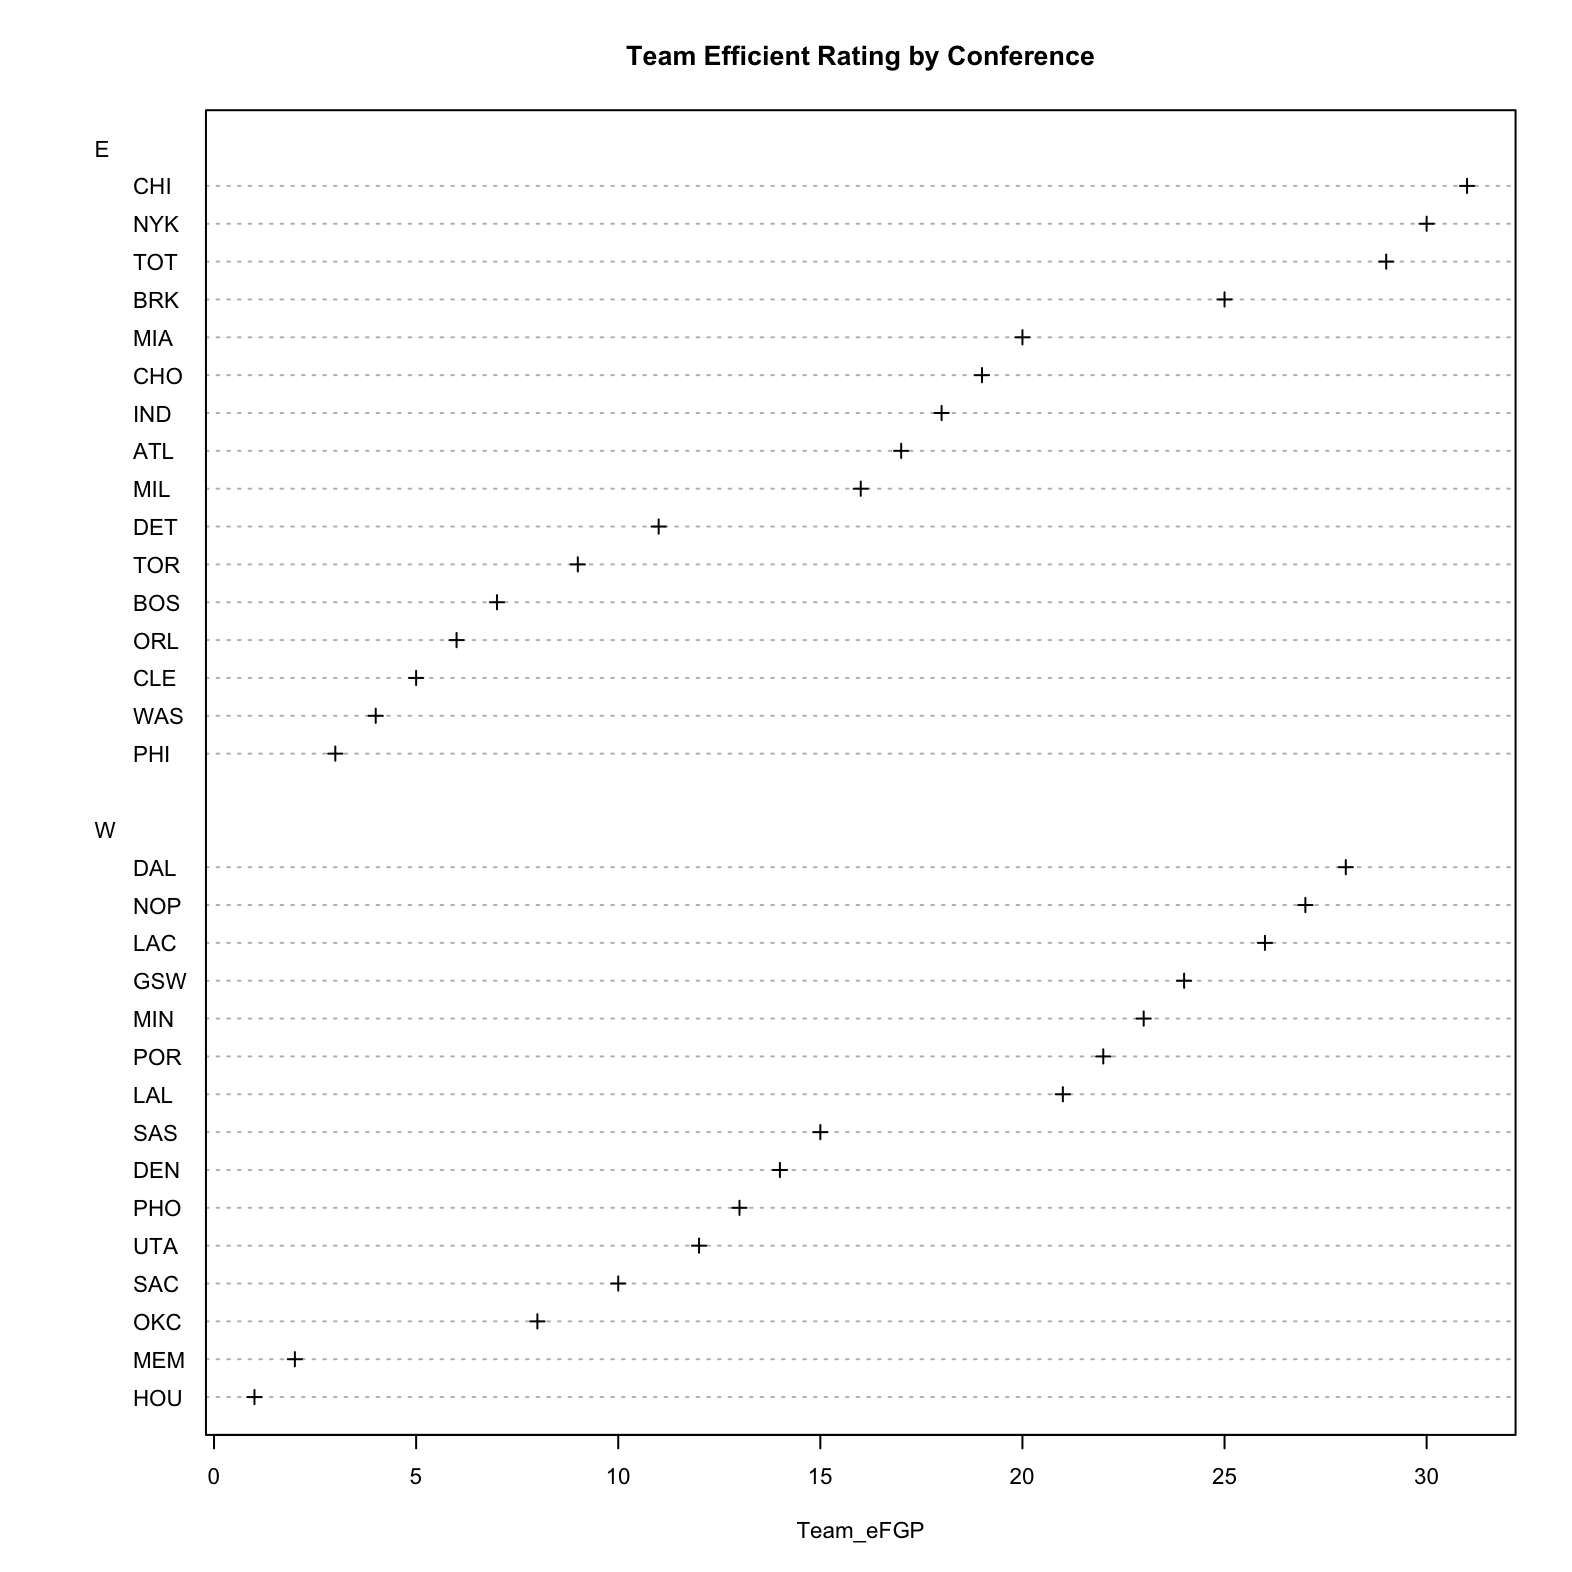
\includegraphics[width=0.9\linewidth, height=5cm]{eFGPdotp.png}
		\caption{有效得分率散点图}
		\label{fig:11}
	\end{subfigure}
	\caption{有效得分率统计描述}
\end{figure}

%第六个变量
\item {\bfseries 球队球员实际命中率Team\_TSR描述性统计分析}左图\ref{fig:12}详细描绘了每个地区的球队球员的实际命中率率的分布情况,可以看出实际命中率变量各个地区的中位数差距不大,但是亚特兰大地区和西南地区的分布差距较大,东南地区存在极端值,其他地区球队球员实际命中率的分布较为集中;右图\ref{fig:13}详细列出了东部地区和西部地区所有队伍球员的实际命中率变量的排名情况, 球员实际命中率最高的球队是西部的新奥尔良黄蜂
, 东部的纽约尼克斯和芝加哥公牛,多伦多猛龙队。

\begin{figure}[h!]
	
	\begin{subfigure}{0.5\textwidth}
		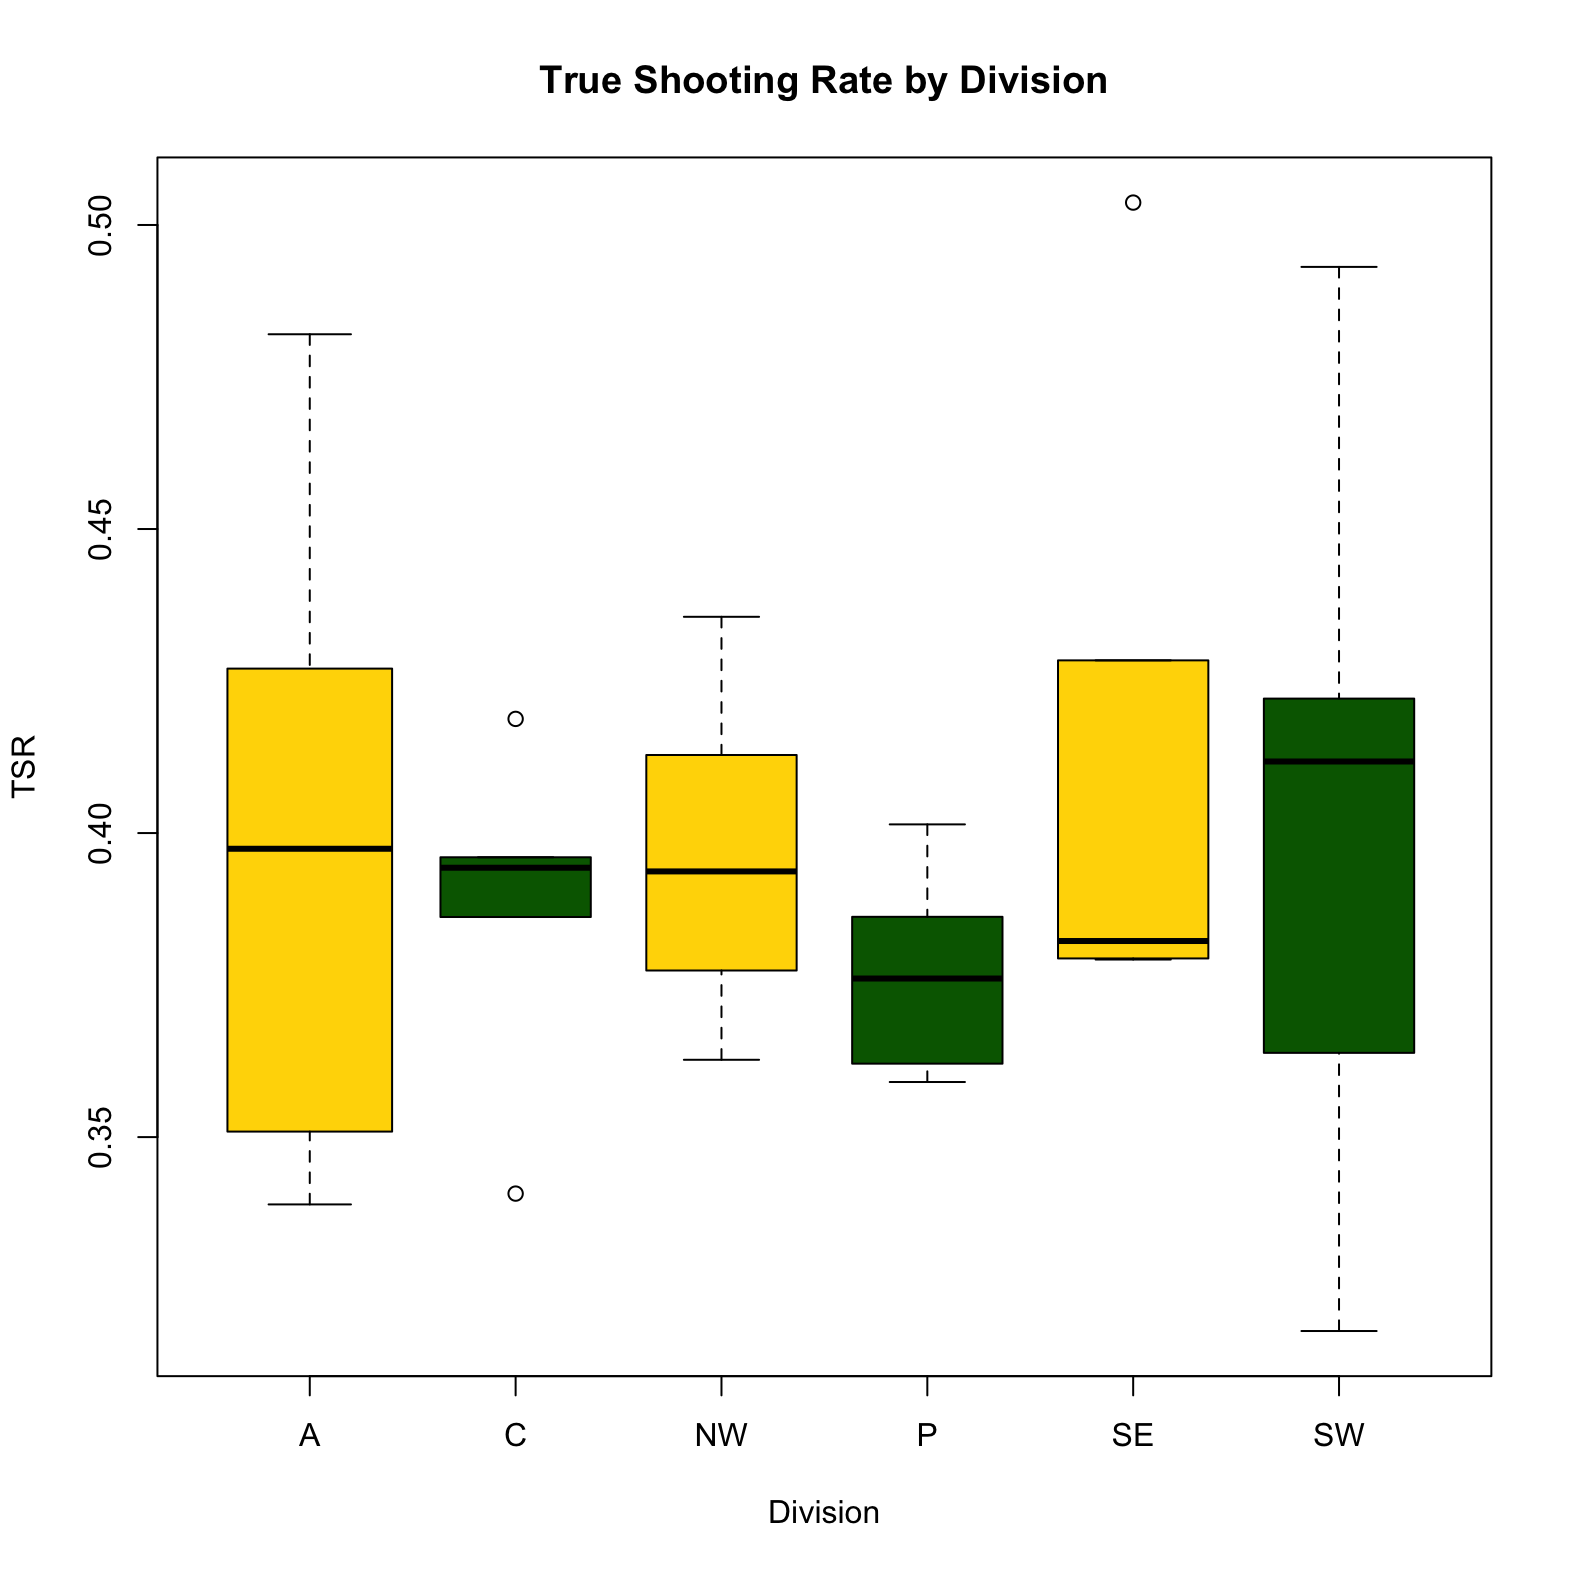
\includegraphics[width=0.9\linewidth, height=5cm]{TSRbp.png} 
		\caption{实际命中率箱线图}
		\label{fig:12}
	\end{subfigure}
	\begin{subfigure}{0.5\textwidth}
		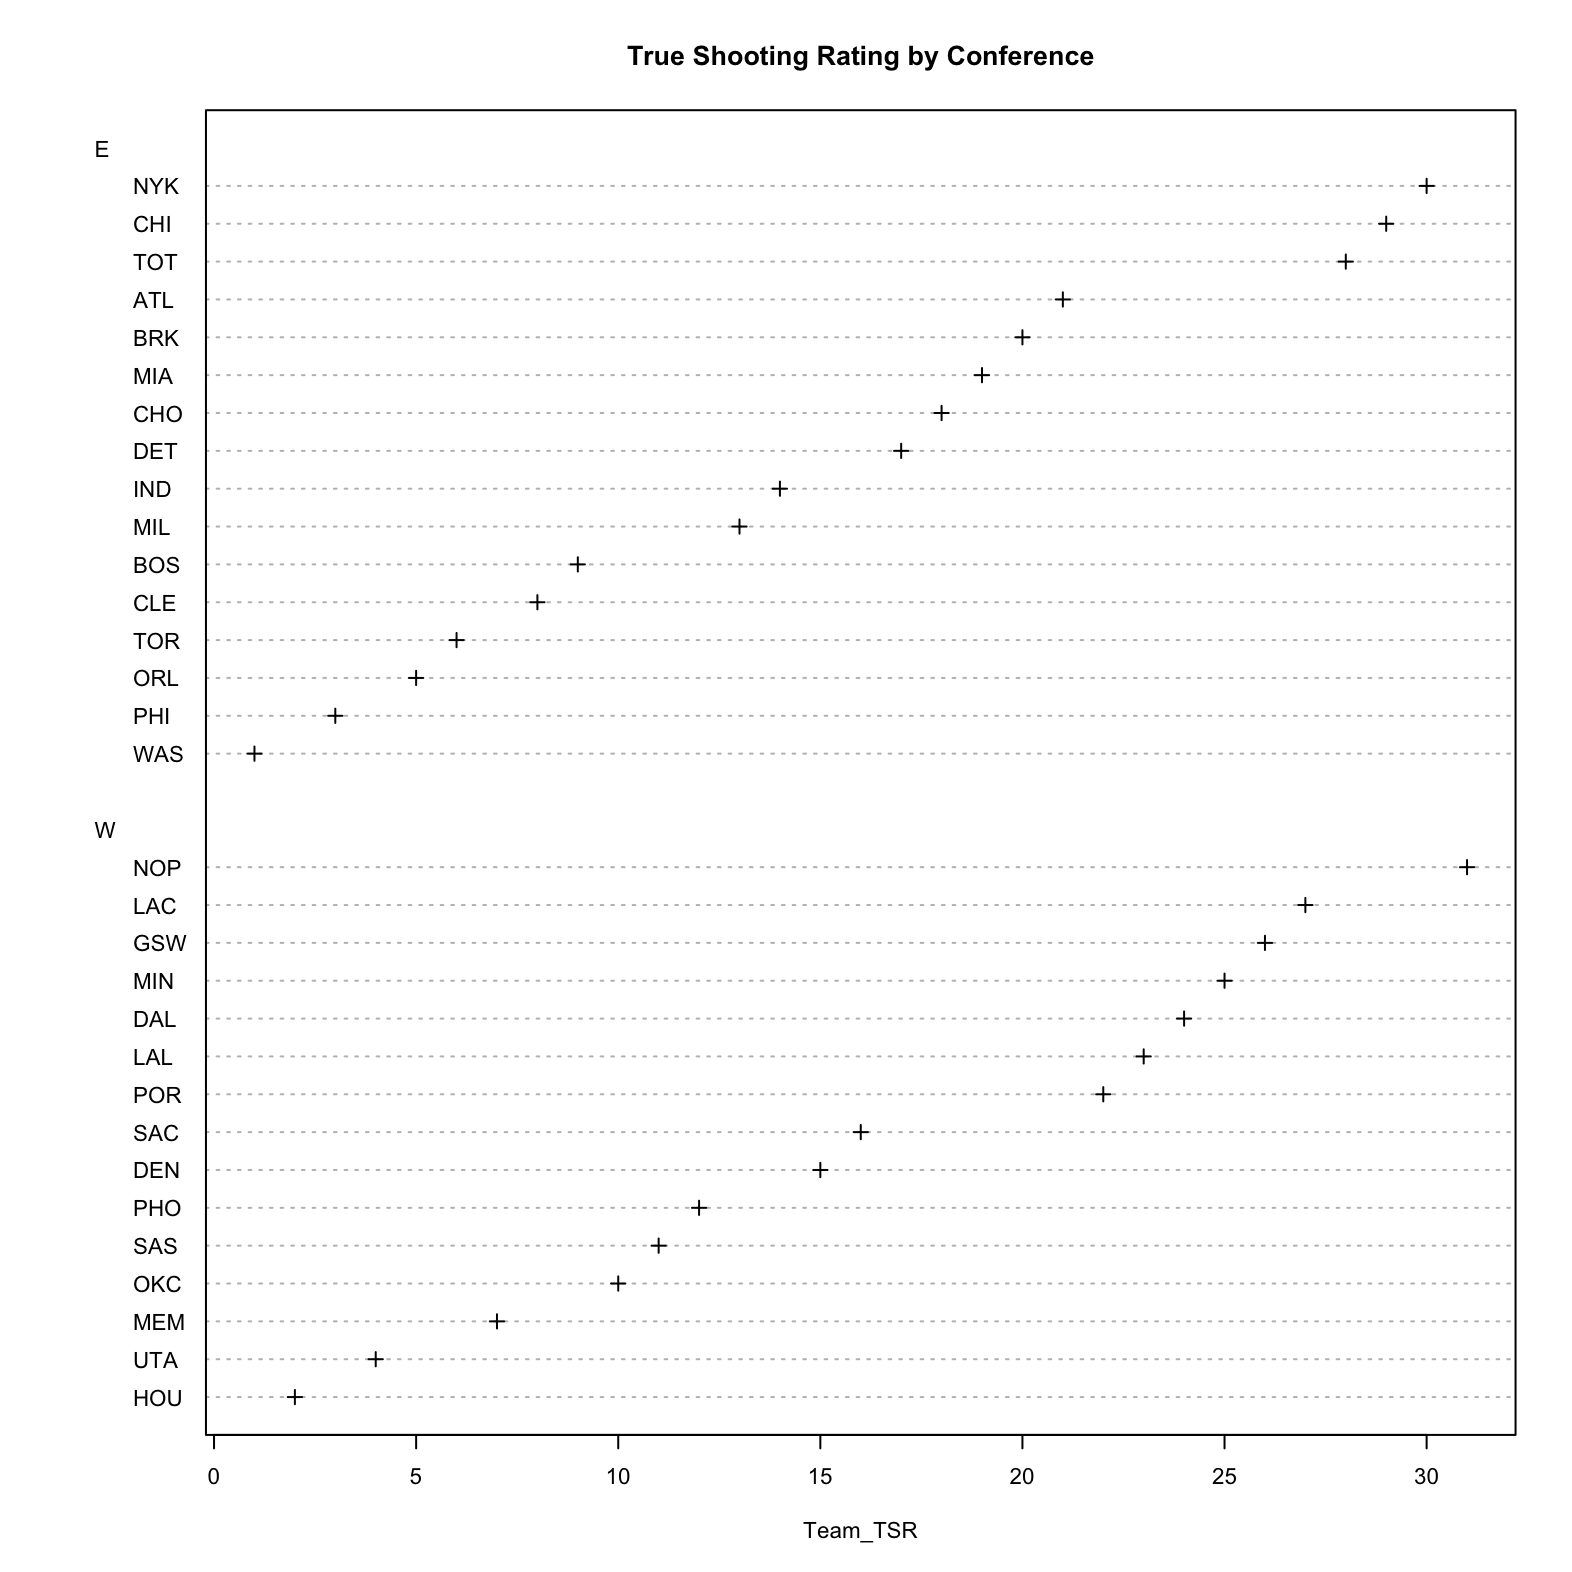
\includegraphics[width=0.9\linewidth, height=5cm]{TSRdotp.png}
		\caption{实际命中率散点图}
		\label{fig:13}
	\end{subfigure}
	\caption{实际命中率统计描述}
\end{figure}


%第7个变量
\newpage
\item {\bfseries 球队球员利用率Team\_USR的统计描述}左图\ref{fig:14}详细描绘了每个地区的球队球员利用率的分布情况,可以看出各地区的球员利用率差距较大,其中西南地区球队的球员利用率变量分布情况较离散,西北地区和东南地区的球队的球员利用率分布情况较为集中。球员利用率变量中位数最高的地区是太平洋地区; 右图\ref{fig:15}详细列出了东部地区和西部地区所有队伍球员利用率变量的排名情况,西部地区的克利夫兰骑士队拥有最高的球员利用率。
\begin{figure}[h!]
	
	\begin{subfigure}{0.5\textwidth}
		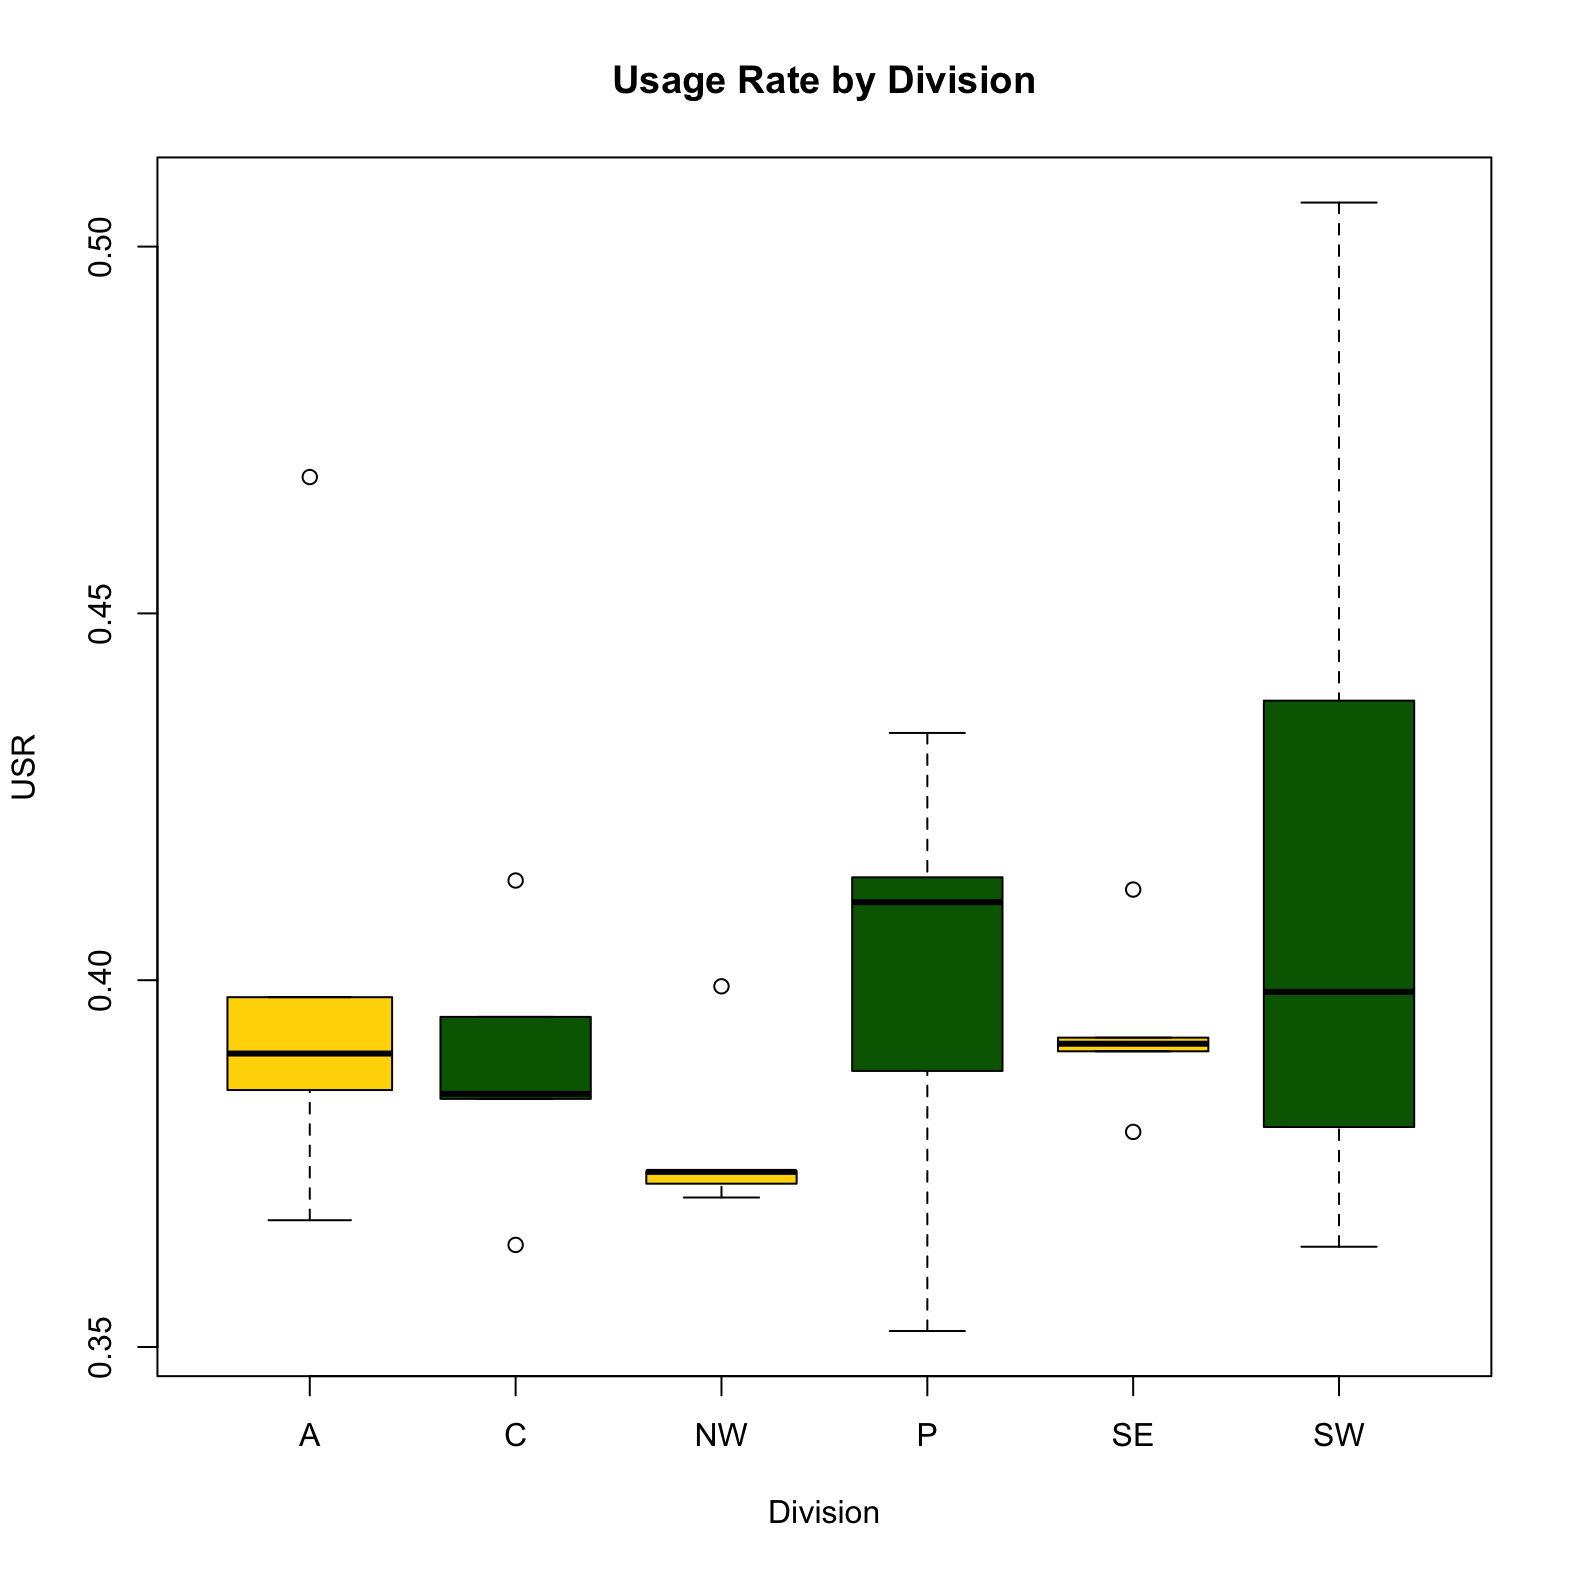
\includegraphics[width=0.9\linewidth, height=5cm]{USRbp.png} 
		\caption{球员利用率箱线图}
		\label{fig:14}
	\end{subfigure}
	\begin{subfigure}{0.5\textwidth}
		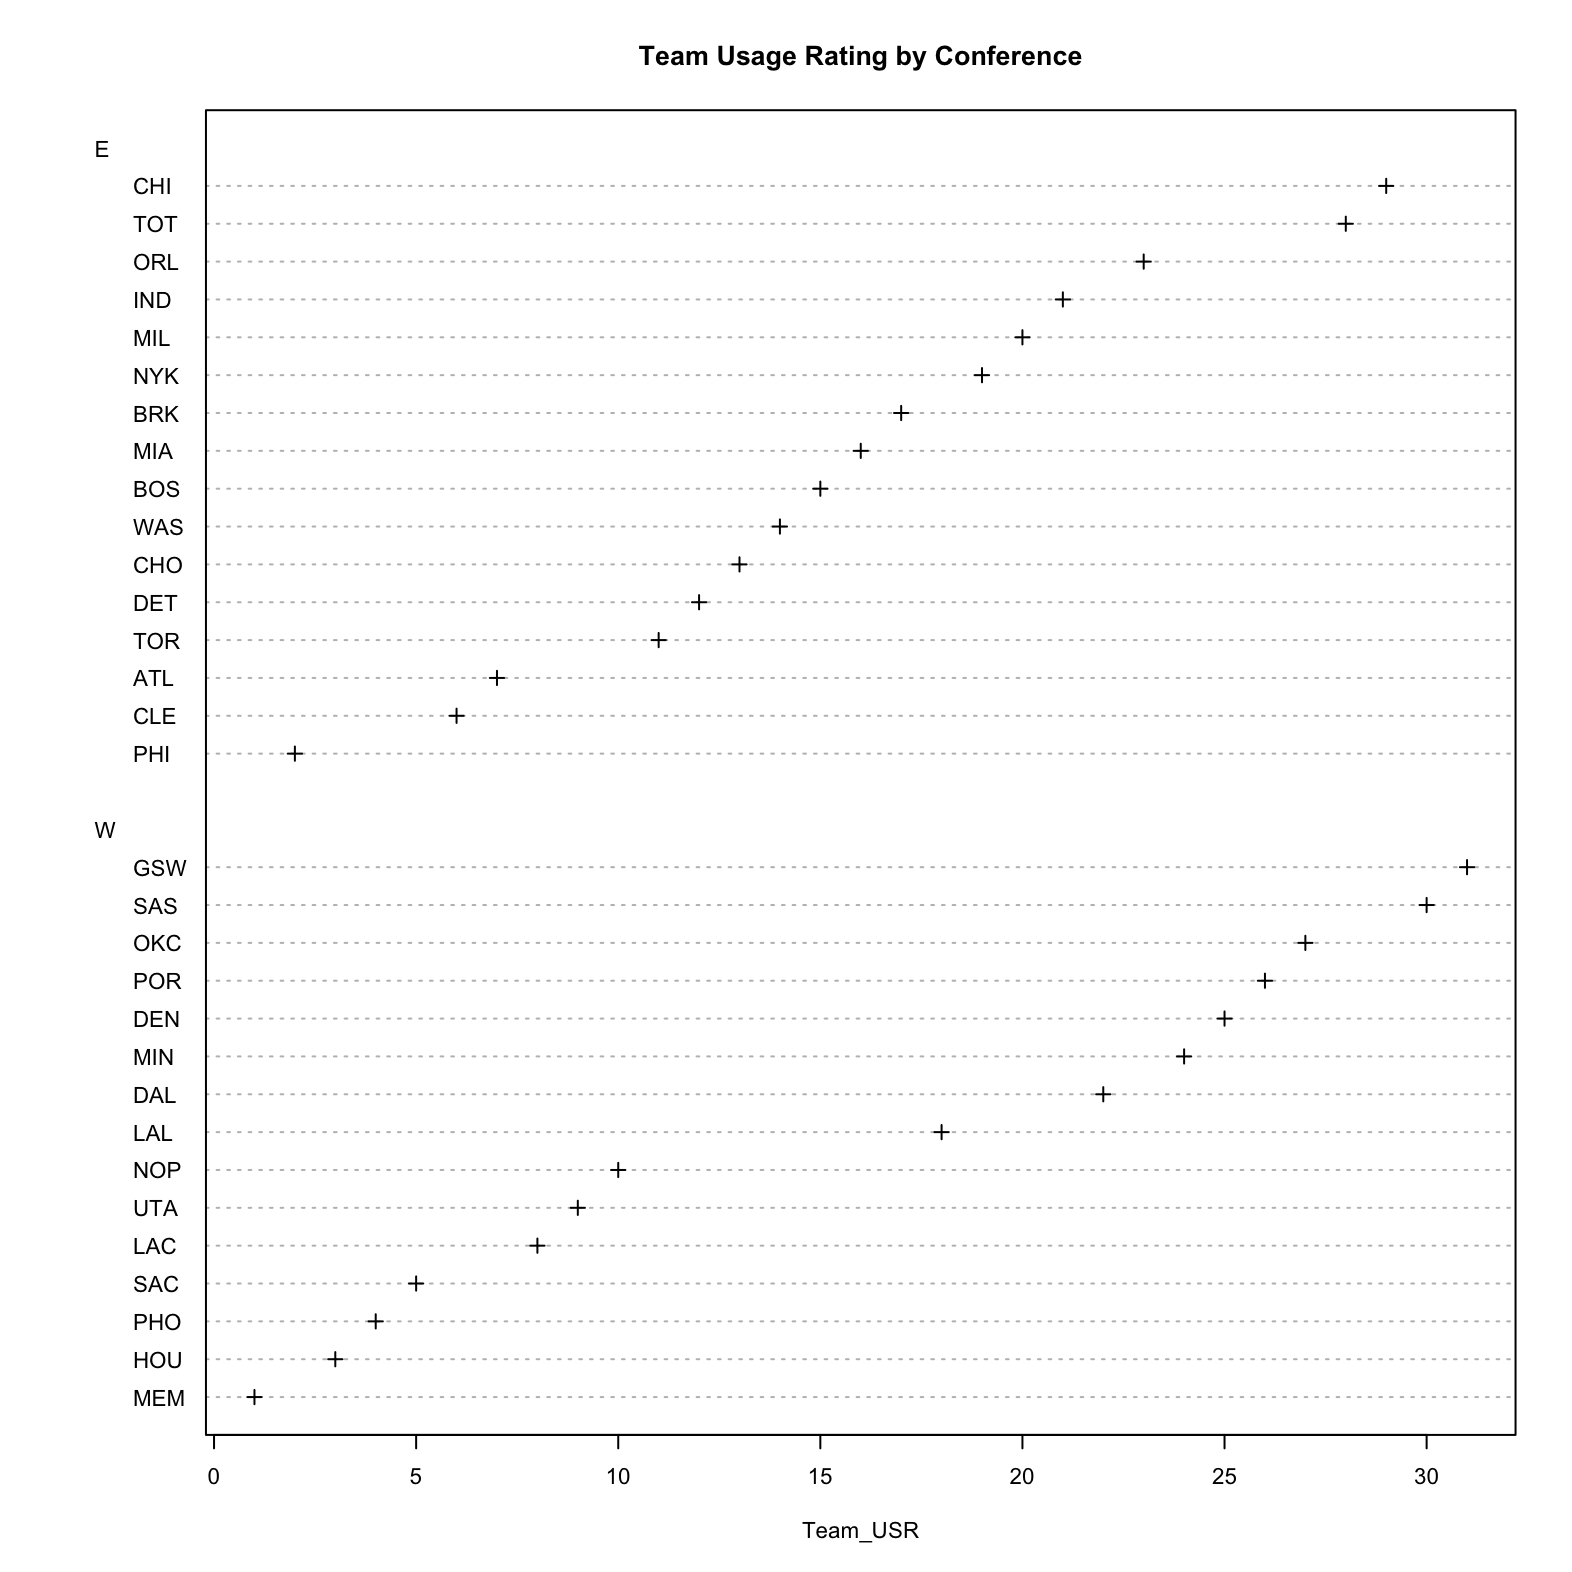
\includegraphics[width=0.9\linewidth, height=5cm]{USRdotp.png}
		\caption{球员利用率散点图}
		\label{fig:15}
	\end{subfigure}
	\caption{球员利用率统计描述}
\end{figure}

	\end{enumerate}






计算指标的均值,中位数,标准差,最大最小值如下表\ref{tab:3}
	\begin{table}[h!]
	\centering
	\begin{tabular}{|c|c|c|c|c|c|}
		\hline
		变量名	          &       Mean &     Median &        Sd         &Max     &    Min\\
		\hline
		W/L\%   &     0.5066452  & 0.5120000 &0.14895694  & 0.7320000 &  0.2070000\\
		MOV/A   &    0.1777419 & -0.4000000 &4.73044164   &8.0500000 & -9.3900000\\
		ORtg/A&    111.1574194 &111.2900000 &2.97113779 &116.6000000 &105.3100000\\
		DRtg/A   & 110.9838710 &110.9700000 &2.91391224 &118.6400000 &105.9400000\\
		NRtg/A     & 0.1719355 & -0.3600000 &4.72743159 &  7.6600000 & -9.8200000\\
		Team\_TSR   & 0.3960872 &  0.3862271 &0.04288839  & 0.5036835  & 0.3181109\\
		Team\_eFGP  & 0.4028148  & 0.4006380 &0.06063737  & 0.5459727   &0.3060132\\
		Team\_USR   & 0.3960933 &  0.3903063 &0.03155086   &0.5060015 &  0.3521769\\
		Team\_PER  &  0.3952573 &  0.3985277& 0.03407403 &  0.4677711 &  0.3392575\\
		Team\_Poss &102.3579355& 102.3520000& 0.34456368 &102.8720000 &101.6280000\\
		\hline
	\end{tabular}
	\caption{描述统计分析}
	\label{tab:3}
\end{table}

胜率的最小值是0.2,最大值是0.7说明最优秀的球队在比赛中有70\%的可能性获胜,最差的球队在比赛中有20\%的获胜率,标准差是0.14,中位数和均值是0.5;说明一般球队的胜率是50\%,也就是这些球队的水平是中间位置,比他强和弱的球队各占50\%。
 比分差距变量最大值是8分,最小值是-9分,即一个球队平均最高可以以8分的差距胜出,最小可以以9分的差距失败,平均水平是0分。标准差是4.73分,即球队之间比分差距变量的分布差距较大。
攻击效率的最高值可达每100次进攻116分,最低不低于每100次进攻105分,平均水平在每100次进攻可获得110分,标准差是3分,即每个球队进攻得分相差不大。
	 防守效率最高可达118分,最低不低于105分,代表对方球队每进攻100次,可以得到118分,最低可得到105分。中位数是110分。标准差是3分,即每个球队的防守失分相差不大。
	 净得分与比分差距的含义相似,分布也相似,在这里可以怀疑这两个变量具有很高的相关性。
	球队球员的实际命中率的平均值是0.39,说明一个球队的球员每投一次球平均有30\%的可能性投进,最高值可达50\%,说明这个优秀的球队每个球员平均都有50\%可能性投篮命中,最低不低于0.3,说明这个球队球员平均只有30\%的可能性投进。标准差是0.04,说明球员实际命中率指标的差距不大。
	球员有效得分率的中位数是0.4,最大值是0.54,说明一个优秀的球队每个球员得分效率可达54\%,最小值是0.31,一个较差的球队得分效率不低于31\%,标准差是0.06,说明球员得分效率变量个体之间差距不大。
	 球队球员利用率平均值是0.39,最大值是0.55,说明这个球队球员在控球时球队对其利用率是55\%,最小值是0.30,一个较差的球队球员在控球时球队对其的利用率不低于30\%,标准差是0.03说明球队之间球员利用效率差距不大,分布较为集中。
	 球队球员效率的平均值是0.39,最大值是0.46,说明球队球员的效率最高平均可达0.46,最小值是0.33说明球队球员的效率最低不低于0.33。
	%插入表格

	
